\chapter{Identification des facteurs influençant l'efficacité du Neurofeedback} \label{ch-saob}

\section*{Introduction}

La réplication et la mise à jour de la méta-analyse de \citet{Cortese2016} décrite dans le chapitre précédent a permis de mettre en évidence la forte 
hétérogénéité des études incluses dans ce type d'analyse. En effet, même si ces études satisfont toutes des critères définis par les auteurs pour pouvoir
les inclure dans leur analyse, elles diffèrent d'un point de vue technique et méthodologique : elles ont été rassemblées sans tenir compte, par exemple, 
de la qualité de l'acquisition de l'\gls{eeg}, du neuromarqueur entrainé lors du \gls{nfb} et du design de l'étude clinique (notamment le nombre de sessions 
et la durée du traitement). 

Afin de mieux identifier l'importance de ces facteurs sur l'efficacité du \gls{nfb}, une nouvelle approche a été implémentée : l'analyse systématique des biais 
(\gls{saob} en anglais). Dans cette analyse, l'efficacité du traitement est considérée comme la variable dépendante expliquée par des variables indépendantes 
qui sont ici les facteurs méthodologiques et techniques. Le but de cette analyse est donc de déterminer les paramètres qui ont une influence sur la performance du 
\gls{nfb} afin de mieux les prendre en compte dans l'implémentation d'études cliniques évaluant l'efficacité de ce traitement. 
\clearpage

\section{Extraction et pré-traitement des facteurs}

La première étape de la \gls{saob} est d'obtenir les facteurs des études sélectionnées. Une liste de facteurs ayant potentiellement une influence sur 
l'efficacité du \gls{nfb} a été établie en \ref{choix_des_facteurs}. Ces facteurs ont ensuite été extraits de chaque étude. Avant de débuter l'analyse, ils ont été pré-traités en 
suivant les étapes décrites en \ref{preprocessing}. 

\subsection{Choix des facteurs} \label{choix_des_facteurs}

Tout d'abord, une revue de littérature et des discussions avec des experts du \gls{nfb} appliqué aux enfants \gls{tdah}, en particulier le Dr. Jean-Arthur Micoulaud Franchi
et le Dr. Louis Mayaud, ont permis de déterminer les facteurs dont il serait intéressant d'étudier l'influence \citep{Vernon2004, Arns2009, Arns2014, 
Cortese2016, Enriquez2017, Strehl2014}. Les facteurs 
spécifiques à l'entrainement par \gls{nfb} sont définis avec plus de précision en \ref{principe_nfb}.

Les paramètres ayant une possible influence sur l'efficacité perçue du \gls{nfb} ont été répartis en cinq catégories :
\renewcommand{\labelitemi}{$\bullet$}
\begin{itemize}
\item \emph{les biais méthodologiques :} 
    \begin{itemize} 
		\item la présence d'un groupe contrôle, 
		\item l'aveugle des évaluateurs (\gls{pblind}), 
		\item la randomisation des sujets dans les essais contrôlés,
		\item l'autorisation de conduire l'étude par un \gls{cpp} (\gls{irb} en anglais).
    \end{itemize}
Ces paramètres ne sont pas spécifiques de l'entrainenement par \gls{nfb} mais pourraient avoir une influence sur les résultats.
En effet, \citet{Ros2019} appellent notamment à employer un groupe contrôle et à avoir recours à des évaluateurs aveugles afin d'améliorer la qualité des études.

Le fait qu'une étude soit validée par un \gls{irb} rend compte de la qualité de l'implémentation méthodologique : les études qui en sont dépourvues sont
condidérées comme étant d'une qualité moindre et donc plus sujettes aux divers biais d'implémentation.  
\item \emph{la population :} 
    \begin{itemize}
    \item la prise de psychostimulants durant le traitement par \gls{nfb}, 
		\item la tranche d'âge des enfants inclus, 
		\item la sévérité des symptômes du TDAH à pré-test (score clinique à pré-test divisé par le score maximal à atteindre sur l'échelle clinique), 
		\item le degré d'engagement dans l'entrainement par \gls{nfb} (observance thérapeutique et ressenti vis à vis du traitement).
    \end{itemize}
Certaines de ces caractéristiques ont déjà été indivividuellement étudiées, en particulier l'impact de la prise de psychostimulants durant l'entrainement par \gls{nfb} dans
\citet{Cortese2016} et ses mises à jour (\citep{Bussalb2019clinical} et celle présentée en \ref{selection_studies}) et également discutées par \citet{VanDoren2017}.
\item \emph{l'implémentation du \gls{nfb} :} 
    \begin{itemize}
    \item le protocole utilisé (\gls{scp}, \gls{smr}, l'augmentation du rythme theta, l'augmentation du rythme beta dans les aires centrale ou frontale 
    et la diminution du rythme theta), 
		\item la présence d'une phase de transfert lors de l'entrainement par \gls{nfb} (bloc durant lequel aucun \textit{feedback} n'est délivré), 
		\item l'utilisation d'une méthodologie de transfert d'apprentissage (pour s'entrainer à la maison ou à l'école), 
    \item le type de seuillage pour les récompenses discrètes (le seuil qui permet l'attribution des récompenses peut avoir une valeur fixe tout au long du traitement ou bien variable
		selon les performances de l'enfant), 
		\item le nombre de sessions de \gls{nfb}, 
		\item la durée et la fréquence des sessions, 
		\item la durée du traitement, 
		\item l'individualisation des bandes de fréquence basée sur l'\gls{iapf} (l'\gls{iapf} est la valeur du pic dans la bande alpha qui diffère selon les individus), 
		\item le couplage du \gls{nfb} avec l'\gls{emg}-Biofeedback (un retour est donné sur l'activité électrique du cerveau, mais aussi sur l'activité musculaire qui est 
		également enregistrée : l'enfant doit
		contrôler les deux simultanément).
		\end{itemize}
Il existe différents types de protocoles dont l'efficacité clinique a déjà été comparée précisément
\citep{Leins2007, Heinrich2019}. Les paramètres concernant l'aide au tranfert d'apprentissage semblent jouer un rôle important comme le soulignent \citet{Arns2014, Gani2008, Strehl2006}.
Par ailleurs, l'influence de ces facteurs sur le \gls{nfb} est étudiée à travers la méta-analyse de \citet{Cortese2016} et ses mises à jour en regroupant les études suivant un protocole standard
\citep{Arns2014}.

La question du seuil est également déterminante comme soulignée par \citet{Arns2014, Strehl2014} tout comme l'importance d'aider au transfert de l'auto-régulation cérébrale
apprise durant les séances de \gls{nfb} à la vie de tous les jours. 

En ce qui concerne le nombre de sessions, ce paramètre a fait l'objet de plusieurs analyses \citep{Cortese2016, Arns2009,
Arns2014, Enriquez2017} afin de déterminer sa valeur optimale. 

La durée du traitement et des sessions ainsi que leur fréquence étant variables d'une étude à l'autre, il parait important
de les étudier \citep{Enriquez2017}. 

Enfin l'individualisation des bandes de fréquences et le couplage entre le \gls{nfb} et l'\gls{emg}-Biofeedback font l'objet de plus en plus d'études \citep{Bioulac2019, Bazanova2018, Bink2014,
Duric2012, Enriquez2017, Klimesch1999}, ainsi leur influence serait intéressante à explorer. 
\item \emph{la qualité de l'acquisition :} 
    \begin{itemize}
    \item la présence de plus d'une électrode d'enregistrement de l'\gls{eeg} (c'est à dire les électrodes qui enregistrent l'\gls{eeg} et d'où 
		est extrait le neuromarqueur qui mènera au \textit{feedback}) et la qualité de 
		l'\gls{eeg}. Cette dernière est représentée par un indicateur allant de 1 à 3, calculé sur les critères suivants : 
        \begin{description} 
        \item[le type d'électrode utilisée :] les électrodes à gel,
        \item[le contrôle de l'impédance :] la vérification du bon contact entre la peau et les électrodes en gardant l'impédance inférieure à $40$k$\Omega$,
        \item[la certification du matériel hardware utilisé :] le matériel doit être conforme à la norme ISO-60601-2-26 \citep{ISO}.
        \end{description}
    Un score de qualité de 3 est donné si tous les critères ci-dessus sont remplis. Si au moins l'un d'eux est satisfait, le score est de 2, sinon il est mis à 1.
		\end{itemize}
Le matériel utilisé semble intuitivement être central quant à l'efficacité du \gls{nfb} d'où notre idée d'étudier son impact de plus près \citep{Lopez2014}. En particulier,
il a été montré que les études sur le \gls{nfb} sont très hétérogènes quant au nombre et au placement des électrodes enregistrant le signal \gls{eeg} sur 
lequel est calculé le \textit{feedback} \citep{Enriquez2017, Rogala2016}.
\item \emph{la qualité du signal} : 
    \begin{itemize}
    \item le rejet en temps réel (l'époque est exclue, pas de retour ou \emph{feedback} calculé) ou la correction (retour calculé sur l'époque débruitée) des 
artefacts oculaires (\gls{eog}),
    \item le rejet en temps réel d'artefacts génériques détectés grâce à leur large amplitude. 
    \end{itemize}
Le signal \gls{eeg} est l'élement central du \gls{nfb} et peut être très facilement contaminé par des artefacts comme expliqué en \ref{steps_NFB_taining} \citep{Chavez2018}, 
ainsi l'effet de la correction ou du rejet 
d'artefacts est à étudier. 
\end{itemize}

Afin d'éviter tout biais d'analyse, le nom des facteurs a été caché durant toute l'analyse : il n'a été révélé qu'à la phase d'interprétation du modèle, lorsque ce dernier a été considéré 
comme valide notamment au niveau de la normalisation des variables et de la validation des hypothèses du modèle.  

\subsection{Pré-traitement des facteurs} \label{preprocessing}

Les auteurs des études incluses dans la \gls{saob} ne précisent pas systématiquement toutes les valeurs des facteurs, ce qui conduit à des observations manquantes. 
Afin que les paramètres pour lesquels peu d'observations sont disponibles ne faussent l'analyse, il est apparu raisonnable de considérer qu'au-delà de 20\%
d'observations manquantes ce paramètre est exclu. Les observations manquantes dans les facteurs comportant des valeurs numériques sont 
imputées et remplacées par -1 pour le \glsfirst{dt} de régression et par la moyenne des valeurs du facteur pour la \glsfirst{wls} et le \glsfirst{lasso}, méthodes décrites en \ref{saob_method}. 

Par ailleurs, comme cette analyse tire avantage de l'hétérogénéité des études, si un facteur a plus de 80\% d'observations identiques, 
celui-ci est également rejeté. 

Ces valeurs de seuil de 20\% et de 80\% ont été choisies arbitrairement.

Il est important de noter qu'une étude ne correspond pas nécessairement à une observation : lorsque plusieurs échelles cliniques et/ou évaluateurs sont disponibles dans une étude,
chaque couple échelle clinique-évaluateur est considéré comme une observation.

Ensuite, les facteurs qui sont des variables catégorielles (le protocole utilisé par exemple) sont codés en \textit{dummies} : la présence du facteur est représentée par un 1 et son absence par 0. 

Enfin, les variables sont standardisées : à chaque observation est soustraite la moyenne de l'ensemble des observations, le tout divisé par l'écart-type de la moyenne de 
l'ensemble des observations. La standardisation a été choisie plutôt que la normalisation afin de garder les valeurs extrêmes dans la \gls{saob} qui auraient été mises à 0 ou 1 avec 
la normalisation. 

Les facteurs sélectionnés et prétraités sont les variables indépendantes de l'analyse.

\section{Explication de l'efficacité du Neurofeedback par des méthodes multivariées}

Afin de déterminer quels facteurs parmi ceux sélectionnés précédemment ont une influence sur l'efficacité du \gls{nfb}, la \gls{saob} utilise trois méthodes multivariées : 
la \gls{wls}, le \gls{lasso} et le \gls{dt}. Ces méthodes ont pour but d'expliquer l'efficacité du \gls{nfb}, quantifiée par un \gls{es}
défini par la suite, à l'aide des facteurs. Les résultats de chaque méthode vont être combinés pour identifier quels paramètres sont susceptibles 
d'avoir un impact sur l'efficacité du \gls{nfb} appliqué aux enfants \gls{tdah}. 

\subsection{Calcul de la taille d'effet intra-groupe} \label{es_within}

L'efficacité du traitement est quantifiée par l'\gls{es}-intra-groupe. Celui-ci est calculé à partir des moyennes et écart-types des scores 
cliniques totaux donnés par les parents et les enseignants (considérés comme \gls{pblind} \citep{Sonuga-Barke2013, Micoulaud2014, Cortese2016}) aux enfants inclus dans 
l'étude à pré et à post-test. De plus, 
lorsqu'une étude fournit des résultats pour plus d'une échelle clinique, l'\gls{es}-intra-groupe est calculé pour chaque échelle :
\begin{equation}
\label{eq:factors_effect_size_within_subject}
\text{ES-intra-groupe} = \frac{M_{\text{post},T} - M_{\text{pré},T}}{\sqrt{\frac{\sigma_{\text{pré},T}^2 + \sigma_{\text{post},T}^2}{2}}},
\end{equation} 
\noindent où $M_{\text{t},T}$ est la moyenne sur l'échelle clinique, pour le traitement $T$, au moment t (pré-test ou post-test) et $\sigma_{\text{t},T}$ représente
son écart-type. Au contraire de l'\gls{es}-inter-groupes défini à l'équation Eq.~(\ref{eq:metareview_effect_size_between}), cet \gls{es} permet de se concentrer sur l'effet du 
traitement au sein du groupe \citep{Cohen1988}. Cette définition de l'\gls{es} a déjà été précédemment utilisée dans la littérature sur le \gls{nfb} 
appliquée aux enfants \gls{tdah} \citep{Arns2009, Maurizio2014, Strehl2017}. Plus la valeur absolue de \gls{es}-intra-groupe est élevée, plus
le traitement étudié est efficace. 

Afin de limiter l'influence d'observations extrêmes parmi les valeurs des \gls{es}-intra-groupe, celles se trouvant à plus de 3 écart-types de la moyenne
de tous les \gls{es}-intra-groupe calculés ont été retirées de l'analyse \citep{Shewhart1931}.

Par la suite, l'ensemble des \gls{es}-intra-groupe est considéré comme la variable dépendante que les variables indépendantes (les facteurs) vont expliquer. 

\subsection{L'analyse systématique des biais} \label{saob_method}

La \gls{saob} a pour but d'identifier les facteurs ayant une influence sur l'efficacité du \gls{nfb} appliquée aux enfants \gls{tdah}. 
Cette analyse comporte trois méthodes qui ont été implémentées à l'aide des bibliothèques Python Scikit-Learn \citep[version 0.18.1]{Pedregosa2011} et Statsmodels \citep[version 0.8.0]{Seabold2010} : 
\begin{itemize}
    \item une régression linéaire multiple et pondérée (\glsfirst{wls} en anglais) \citep{Montgomery2012},
	  \item une régression linéaire régularisée (\glsfirst{lasso} en anglais) \citep{Tibshirani1996},
	  \item un arbre de décision de régression (\glsfirst{dt} en anglais) \citep{Quinlan1986}.
\end{itemize}

La \gls{wls} a été choisie car son équivalent non pondéré (l'\gls{ols}) est très connue car couramment utilisée. Par ailleurs, cette méthode est très proche de la méta-régression qui est 
parfois mise en place dans les méta-analyses pour quantifier la relation entre un paramètre des études et leur efficacité \citep{Cortese2016, Borenstein2009}. 

Le \gls{lasso} est également une régression mais permet de sélectionner clairement les variables indépendantes ayant une influence sur la variable dépendante. 

Enfin, une méthode non linéaire, le \gls{dt} de regression, est employée car elle permet d'ordonner les variables indépendantes selon leur influence sur la variable dépendante. 
Par ailleurs, un seuil de décision est calculé, ce qui permet d'avoir une idée de la valeur à partir de laquelle le facteur a une influence positive sur l'efficacité du \gls{nfb}.

Les résultats de ces trois méthodes intrinsèquement différentes vont être combinés : si un facteur est identifié par les trois méthodes, alors son influence sur l'efficacité du 
\gls{nfb} est plus probable que si une seule méthode l'identifie. 

Il a été décidé d'utiliser trois méthodes car celles choisies sont suffisammment différentes pour mener à des conclusions intéressantes : si malgré leurs dissimilitudes 
elles sont d'accord sur l'influence d'un facteur alors on peut raisonnablement conclure que cette influence est fortement probable. Il aurait été possible
d'avoir recours à plus de méthodes mais étant donné l'aspect novateur de cette approche, il semblait préférable de ne pas complexifier le message en utilisant trop de méthodes.

\subsubsection{La régression linéaire multiple et pondérée} \label{wls_part}
La régression linéaire a pour but d'estimer les coefficients de régression qui lient linéairement les facteurs aux \gls{es}-intra-groupe \citep{Montgomery2012}. Ici, nous préférerons 
utiliser une régression linéaire pondérée (en anglais, \glsfirst{wls}) afin d'être sensible au fait que toutes les études ne contribuent pas de la même manière. 
En effet, cela permet de prendre en compte que, d'une part, pour certaines études, plusieurs échelles cliniques sont disponibles, et que, d'autre part, les études ont des 
tailles d'échantillon très différentes.

Les coefficients $\hat{\beta}_{j}$, $0 \leq j \leq p$, sont obtenus en minimisant la somme pondérée des erreurs quadratiques :
\begin{equation}
\label{eq:factors_wls-minimization}
\hat{\beta} = \argmin_\beta \sum_{i=1}^{n} w_{i} \Big(y_i - \beta_0 - \sum_{j=1}^{p}\beta_{j}x_{ij}\Big)^2,
\end{equation} 
avec $x_{ij}$ la valeur de l'observation $i$, $1 \leq i \leq n$ sur la variable indépendante $j$, $1 \leq j \leq p$, $\beta_0$ l'ordonnée à l'origine (l'\textit{intercept} en anglais), 
$\beta_j$ est un coefficient de régression et $y_i$ la variable dépendante.
Le poids $w_{i}$ associé à chaque observation $i$ est défini comme suit : 
\begin{equation}
\label{eq:weight_WLS}
w_{i} = \frac{\text{N}_{k}}{\text{NS}_{k}},
\end{equation} 
avec $\text{N}_{k}$  le nombre de sujets dans l'étude $k$ dans le groupe suivant le traitement et $\text{NS}_{k}$  le nombre 
d'échelles cliniques disponibles dans l'étude $k$ évaluant l'efficacité du traitement. Lorsque tous les $w_{i}$ sont égaux à 1, on se retrouve dans le
cas de l'\gls{ols}. La différence entre la régression non pondérée (l'\gls{ols}) et pondérée (la \gls{wls}) sur des données factices est représentée dans le cadre
d'une régression simple à la Figure~\ref{Figure:factors_comparison_ols_wls}.

\begin{figure}[h!]
  \centering
	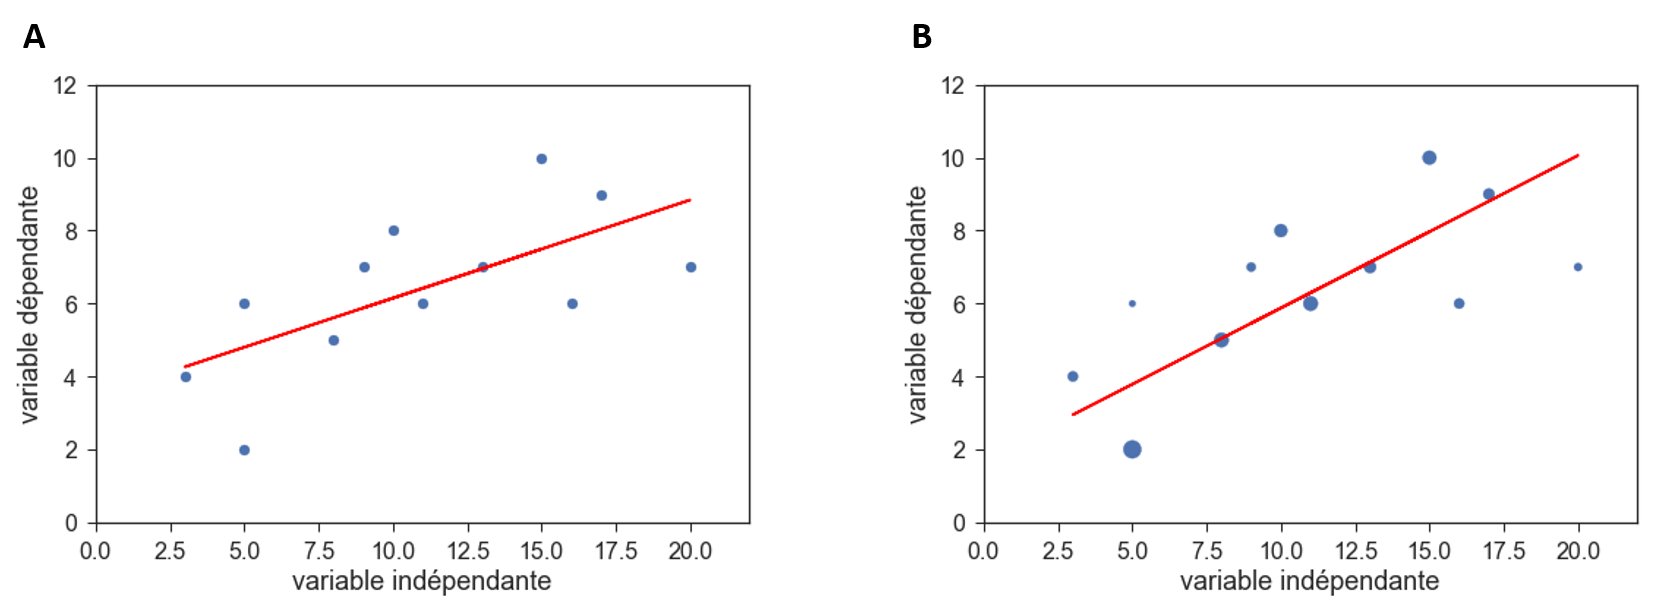
\includegraphics[width=1.0\linewidth]{figures/chapter-3/factors-comparison-ols-wls} 
  \caption[Comparaison des régressions simples non pondérée (\gls{ols}) et pondérée (\gls{wls}) sur des données factices.]{Comparaison des régressions 
	simples non pondérée (\gls{ols}) en \textbf{A} et pondérée (\gls{wls}) en \textbf{B} sur des données factices. Les points bleus correspondent aux observations
	dont la taille dans le cas de la \gls{wls} est proportionnelle au poids qui leur est attribué. Les droites rouges correspondent aux droites de régression : dans le cas de la \gls{wls} elle
	est plus proche des points ayant un fort poids. Dans notre cas la variable dépendante sera l'\gls{es}-intra-groupe et la variable indépendante un facteur.}
  \label{Figure:factors_comparison_ols_wls}
\end{figure}

Sous forme matricielle, la \gls{wls} se traduit ainsi : 
\begin{equation}
\label{eq:factors_model_WLS}
\textbf{W}y = \textbf{WX}\beta + \epsilon.
\end{equation}
$\textbf{X}$ est une matrice inversible $(n \times q)$ et représente $n$ observations sur chaque $p$ variable indépendante et l'\textit{intercept}  
($q = p + 1$), 
$\beta$ est un vecteur $(q \times 1)$ des coefficients de régression associés et l'\textit{intercept}, $\textbf{W}$ est une matrice diagonale $(n \times n)$  
des poids $w_{i}$, $y$ est un vecteur $(n \times 1)$ des variables dépendantes et $\epsilon$ est un vecteur $(n \times 1)$ d'erreurs.

Le but de la \gls{wls} est d'estimer le vecteur de coefficients $\beta$ en minimisant la somme pondérée des carrés des résidus (\gls{wrss} en anglais) :
\begin{equation}
\label{eq:factors_WRSS}
\text{WRSS} = \sum_{i=1}^{n} w_i \Big(y_i - \hat{y}_i\Big)^2, 
\end{equation}
avec $\hat{y}_i = \beta_{0} + \sum_{j=1}^{p}\beta_{j}x_{ij}$, les valeurs prédites.

Une fois le vecteur $\beta$ estimé, on cherche à savoir si les hypothèses du modèle sont vérifiées : 
\begin{itemize}
    \item la matrice ${\textbf{X}}^{T}\textbf{W}^{T}\textbf{WX}$ est régulière (c'est à dire qu'elle est inversible : il existe une matrice \textbf{B} appelée matrice inverse de 
		${\textbf{X}}^{T}\textbf{W}^{T}\textbf{WX}$ telle que B = $({\textbf{X}}^{T}\textbf{W}^{T}\textbf{WX})^{-1}$),
    \item la tendance linéaire estimée est trouvée significative en se basant sur la statistique F,
    \item les résidus sont distribués normalement en se basant sur l'asymétrie (\textit{skewness} en anglais), le Kurtosis et le test Omnibus.
\end{itemize} 

La statistique F est le résultat du test statistique où l'hypothèse nulle est que tous les coefficients de régression sont égaux à 0. Ce test est effectué en calculant 
la statistique F \citep{James2013} :

\begin{equation}
\label{eq:factors_statistic_F}
\text{F} = \frac{ (\text{WTSS} - \text{WRSS}) / p }{ \text{WRSS} /(n - p - 1) }, 
\end{equation}
avec $\text{WTSS} = \sum_{i=1}^{n} w_i(y_i - \bar{y})^2$, la somme totale des carrés des résidus (\gls{wtss} en anglais) et $\bar{y}$ la moyenne 
pondérée par les $w_i$ des $y_i$. 

La $p$-value associée à la statistique F est calculée à partir de la F-distribution, qui est une distribution de probabilités de la statistique F, obtenue si $H_{0}$ 
est vraie et si les résidus sont distribués normalement.

Afin de déterminer si les résidus sont distribués normalement, la \textit{skewness}, le Kurtosis et le test Omnibus sont utilisés \citep{dagostino1973, dagostino1971, Bowman1975}.

La \textit{skewness} $\gamma$ rend compte d'à quel point la forme générale d'une distribution diffère de celle d'une distribution normale : 
\begin{equation}
\label{eq:factors_skewness}
\kappa = E \Big[ \Big(\frac{ Y - \mu }{ \sigma }\Big)^{3} \Big], 
\end{equation}
avec $E$ la valeur attendue, $Y$ la variable aléatoire, $\mu$ la moyenne de la population et $\sigma$ l'écart-type de la population.

La \textit{skewness} d'une distribution normale vaut 0.

En pratique, la \textit{skewness} est estimée dans la population en calculant la \textit{skewness} pour un échantillon. On suppose alors
que la variable aléatoire est distribuée uniformément :

\begin{equation}
\label{eq:factors_skewness_estimation}
g_{1} = \frac{ \mu_{3} } {s^3},
\end{equation}
avec $\mu_{3}$ le troisième moment central de l'échantillon et $s$ l'écart-type de l'échantillon.

Le Kurtosis $\kappa$ quantifie à quel point les formes des queues de la distribution diffèrent par rapport à une distribution normale :
\begin{equation}
\label{eq:factors_kurtosis}
\kappa = E \Big[ \Big(\frac{ Y - \mu }{ \sigma }\Big)^{4} \Big], 
\end{equation}
avec $E$ la valeur attendue, $Y$ la variable aléatoire, $\mu$ la moyenne de la population et $\sigma$ l'écart-type de la population.

Le Kurtosis d'une distribution normale est de 3, cependant le Kurtosis est parfois exprimé en tant qu'excès de Kurtosis :
\begin{equation}
\label{eq:factors_kurtosis_excess}
g_{2} = \frac{ \mu_{4} } {s^4}, 
\end{equation}
avec $\mu_{4}$ le troisième moment central de l'échantillon et $s$ l'écart-type de l'échantillon.

Ainsi, avec les valeurs de kurtosis et de skewness on peut quantifier d'à quel point la distribution des résidus diffère 
d'une distribution normale. Afin de savoir si cette différence est significative, le test Omnibus peut être utilisé. 

Ce test se base sur les valeurs de la \textit{skewness} et le Kurtosis pour tester l'hypothèse $H_{0}$ qui est que les résidus sont distribués normalement.
Pour ce faire, il regroupe les variables aléatoires pour la \textit{skewness} et le Kurtosis en un seul test statistique :
\begin{equation}
\label{eq:factors_omnibus_statistic}
K = Z_{1}(g_{1})^2 + Z_{2}(g_{2})^2, 
\end{equation}
avec $K$ la statistique du test Omnibus, $g_{1}$ la variable aléatoire de la \textit{skewness} et
$g_{2}$ la variable aléatoire de l'excès de Kurtosis, et $Z_{1}$ et $Z_{2}$ des fonctions de transformation qui ont pour but de rendre 
les distributions de $g_{1}$ et $g_{2}$ normales.

Si toutes ces hypothèses sont satisfaites, alors les résultats de la \gls{wls} peuvent être interprétés. A l'aide d'un t-test, on détermine  
parmi les coefficients $\beta_{j}$ où $0 \leq j \leq p$, ceux qui sont significativement différents de 0 (avec un seuil de significativité de 5\%) : 
pour ces coefficients, le facteur qui leur est associé est supposé avoir une influence sur l'efficacité du \gls{nfb}. Par ailleurs, 
le signe du coefficient indique si cette influence est positive ou négative. 

Etant donné le nombre important de variables indépendantes, le pourcentage de variance estimée par la \gls{wls} est quantifié par le coefficient de 
détermination ajusté, $R^2_{adjusted}$ (\textit{adjusted R-Squared} en anglais) plutôt que par le coefficient de détermination simple $R^2$ (\textit{R-Squared} en anglais)
définis respectivement aux équations Eq.~(\ref{eq:factors_R_squared}) et Eq.~(\ref{eq:factors_adjusted_R_squared}) \citep{James2013}.
\begin{equation}
\label{eq:factors_R_squared}
R^2 = \frac{ \text{WTSS} - \text{WRSS} }{ \text{WTSS} }, 
\end{equation}

\begin{equation}
\label{eq:factors_adjusted_R_squared}
R^2_{adjusted} = 1 - \frac{ (1 - R^2) (n - 1) }{ n - p - 1 }, 
\end{equation}
avec $n$ le nombre d'observations et $p$ le nombre de variables indépendantes.


Une régression linéaire ordinaire (\gls{ols} en anglais) est aussi mise en place pour observer l'impact des poids sur les résultats. 

\subsubsection{La régression linéaire avec régularisation parcimonieuse $\ell_1$}

La deuxième méthode appliquée lors de la \gls{saob} est le \glsfirst{lasso} qui intègre la sélection de variables dans le modèle linéaire grâce 
à un a priori de parcimonie des variables/coefficients, obtenue via une régularisation par la norme $\ell_1$ \citep{Tibshirani1996}.

La régression régularisée par la norme $\ell_1$ est préférable ici à la régression \textit{Ridge} \citep{James2013} régularisée par 
la norme $\ell_2$ (aussi appelée régularisation de Tikhonov) : en effet, la norme $\ell_2$ donne des coefficients lissés, alors que la norme $\ell_1$ donne des coefficients parcimonieux 
(i.e., les coefficients utiles sont sélectionnés alors que les autres sont mis à 0). 

Les coefficients $\hat{\beta}_{j}$, $0 \leq j \leq p$ sont obtenus en minimisant le coût :
\begin{equation}
\label{eq:factors_lasso-minimization}
\hat{\beta} = \argmin_\beta \sum_{i=1}^{n} \Big(y_i - \beta_{0} - \sum_{j=1}^{p}\beta_{j}x_{ij}\Big)^2 + \lambda \sum_{j=0}^{p}\abs{\beta_{j}},
\end{equation} 
où $\lambda$ est le paramètre de régularisation qui, en augmentant, met de plus en plus de coefficients à 0. Ce phénomène est illustré à la 
Figure~\ref{Figure:factors_comparison_lasso_ridge_ols_lasso} où est représentée l'évolution de la valeur de chaque coefficient $\hat{\beta}_{j}$ en fonction de
la valeur de $\lambda$ dans le cas des régressions \gls{lasso} (en \textbf{A}) et \textit{Ridge} (en \textbf{B}) sur des données factices. Lorsque $\lambda = 0$, on retombe
sur la solution de l'\gls{ols} évoqué en \ref{wls_part}.

\begin{figure}[h!]
  \centering
	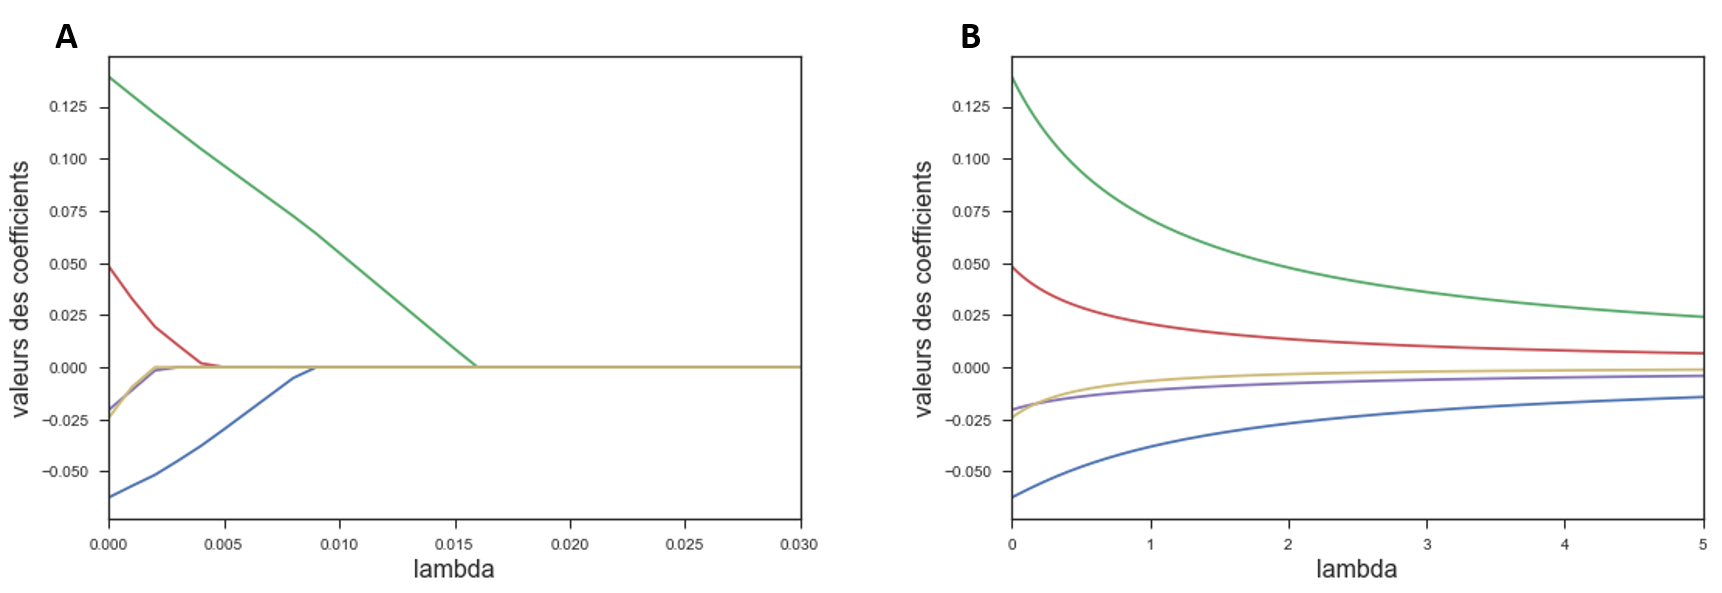
\includegraphics[width=1.0\linewidth]{figures/chapter-3/comparison-lasso-ridge-ols-lasso} 
  \caption[Comparaison des régressions \gls{lasso} et \textit{Ridge} sur des données factices.]{Evolution de la valeur de chaque coefficient $\hat{\beta}_{j}$ (en vert, rouge, jaune, violet et bleu) en fonction de
  la valeur de $\lambda$ dans le cas des régressions \gls{lasso} (en \textbf{A}) et \textit{Ridge} (en \textbf{B}) sur des données factices. Pour $\lambda = 0$, on se retrouve
  dans le cas de l'\gls{ols}. Le \gls{lasso} effectue bien une sélection de variables en mettant à zéro les coefficients les plus faibles.}
  \label{Figure:factors_comparison_lasso_ridge_ols_lasso}
\end{figure}

Le paramètre de régularisation optimal est déterminé par une validation croisée \textit{leave-one-out}. Cette méthode prend une seule observation 
comme donnée de test pour la validation, laissant $n - 1$ observations pour les données d'entraînement. Le processus de la validation croisée est 
ensuite répété $n$ fois pour que chaque observation soit utilisée exactement une fois comme donnée de test. 

Pour chaque itération, appelée \textit{fold} en anglais, l'erreur quadratique moyenne (\gls{mse} en anglais) définie à l'équation Eq.
~(\ref{eq:factors_mse}) est calculée sur les données de test
puis les $n$ résultats sont moyennés pour mener à une seule observation qui permet de trouver le $\lambda$ optimal. Celui-ci correspond à l'abscisse du minimum de la \gls{mse} 
du \textit{fold} moyen calculée sur un large intervalle de $\lambda$ \citep{James2013}. 

\begin{equation}
\label{eq:factors_mse}
\text{MSE} = \frac{1}{n}\sum_{i=1}^{n} \Big(\hat{y}_i - {y}_i\Big)^2,
\end{equation}
avec $\hat{y}$ les valeurs prédites.

Un coefficient non mis à 0 signifie que le facteur associé pourrait avoir une influence sur l'efficacité du \gls{nfb} et, ici aussi, 
le signe du coefficient indique la direction de l'effet.

\subsubsection{L'arbre de décision de régression}

La troisième et dernière méthode utilisée est le \glsfirst{dt} de régression qui, à l'inverse des deux précédentes méthodes, n'est pas une méthode 
linéaire \citep{Quinlan1986}. Elle divise l'ensemble des observations en sous-ensembles de plus en plus petits en se basant sur la présence 
d'une variable qualitative ou sur la comparaison à un seuil appliqué à une variable quantitative. La position de la variable indépendante utilisée (et le
choix du seuil de comparaison dans le cas d'une variable quantitative) pour subdiviser l'ensemble des données est déterminée de façon à minimiser la
\gls{mse} définie à l'équation Eq.~(\ref{eq:factors_mse}) :

La première variable utilisée pour diviser l'ensemble des données se situe dans le noeud racine (\textit{root node} en anglais), les autres
variables qui mènent à une nouvelle subdivision sont dans des noeuds, et les noeuds où la division s'arrête sont appelés
feuilles (\textit{leaf nodes}) de l'arbre. La profondeur de l'arbre peut être définie par le nombre d'observations minimal nécessaire
pour diviser un sous-ensemble ou dans une feuille. Ce critère a été utilisé ici de façon arbitraire : une feuille doit comporter au moins 10\% d'observations. 
Un arbre exemple est schématisé à la Figure~\ref{Figure:factors_decision_tree_example}.

\begin{figure}[h!]
  \centering
	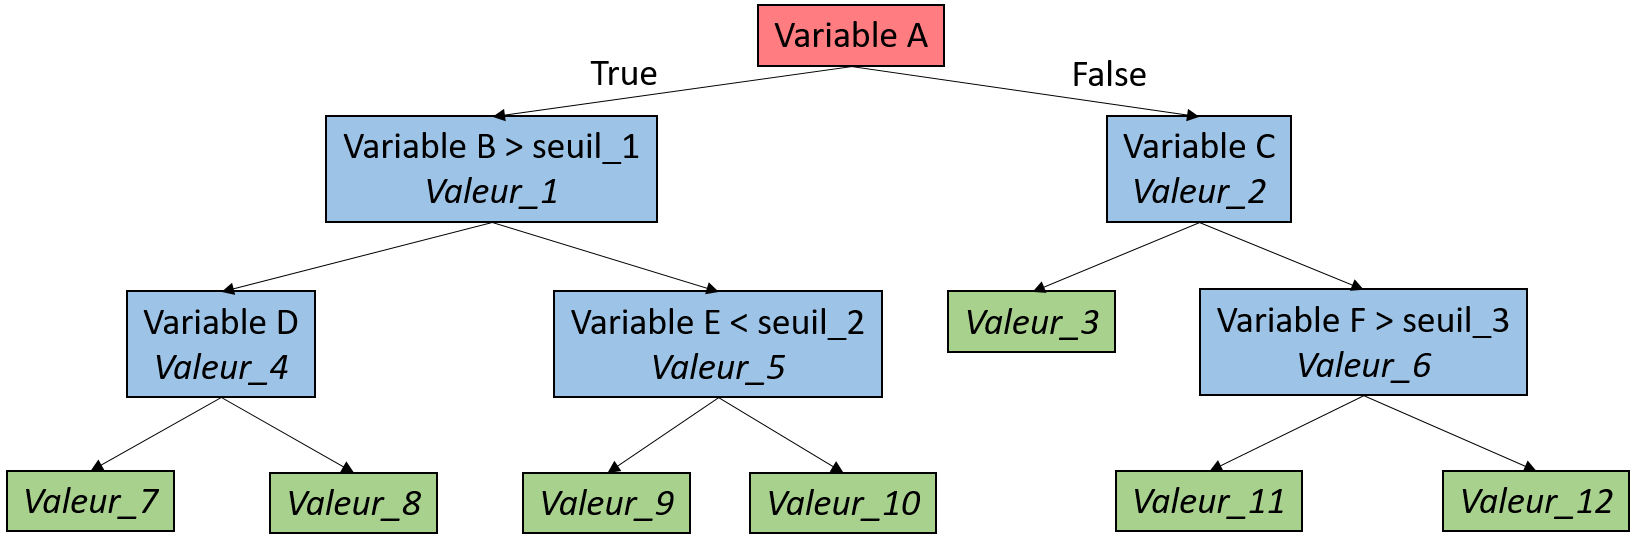
\includegraphics[width=1.0\linewidth]{figures/chapter-3/decision-tree-example} 
  \caption[Exemple schématique d'arbre de décision de régression.]{Exemple schématique d'arbre de décision de régression. Le \textit{root node} est en rouge, les noeuds sont en bleu et les feuilles en vert. 
	Les variables A, C et D sont catégorielles ; les variables B, E et F sont numériques. Les "Valeurs\_X" correspondent à la valeur 
	prédite par l'arbre de décision de la variable dépendante suite à la division précédente.}
  \label{Figure:factors_decision_tree_example}
\end{figure}

Afin que les seuils calculés par le \gls{dt} aient un sens, la variables indépendantes n'ont ici pas été standardisées. Dans le cas de la \gls{saob}, 
les facteurs se retrouvent dans les noeuds : leur influence sur l'efficacité du \gls{nfb} est quantifiée par la valeur de la variable dépendante 
obtenue après chaque division mais aussi par leur place dans l'arbre. En effet, plus un facteur est en haut de l'arbre plus les divisions se font sur un grand nombre
d'observations, ainsi son impact sur l'efficacité est davantage probable.

\section{Analyse des facteurs influençant le Neurofeedback} \label{saob_results}

Les résultats de la \gls{saob} sont présentés ici. Cette méthode, dont les premières étapes (i.e. la sélection des études et le calcul des \gls{es}) rappellent
la méta-analyse, se distingue de cette dernière par l'utilisation de méthodes multivariées. Celles-ci tirent avantage de l'hétérogénéité des études
sur le \gls{nfb} appliqué aux enfants \gls{tdah} pour déterminer les facteurs ayant un impact sur la performance du \gls{nfb}.

\subsection{Sélection des études} \label{saob_selection_studies}

\subsubsection{Méthode de sélection}

Les termes entrés dans Pubmed pour la recherche des articles à inclure dans la \gls{saob} sont :
(ADHD OR adhd OR attention deficit disorder with hyperactivity OR minimal brain disorders OR syndrome hyperkinetic OR hyperkinetic
syndrome OR hyperactivity disorder OR hyperactive child syndrome OR childhood hyperkinetic syndrome OR attention deficit hyperactivity disorders
OR attention deficit hyperactivity disorder OR adhd attention deficit hyperactivity disorder OR addh OR overactive child syndrome OR attention deficit 
hyperkinetic disorder OR hyperkinetic disorder OR attention deficit disorder hyperactivity OR attention deficit disorders hyperactivity OR child 
attention deficit disorder OR hyperkinetic syndromes OR syndromes hyperkinetic OR hyperkinetic syndrome childhood) AND 
(randomized control trial OR RCT OR randomized control study OR Pilot Study OR Study OR Trial OR randomized trial) AND 
(neurofeedback OR “EEG biofeedback” OR neurotherapy OR SCP OR “slow cortical potentials” OR Theta Beta Ratio OR “TBR”). 

Cette recherche est proche de celle conduite dans le chapitre \ref{chapitre-2} lors de la mise à jour de la méta-analyse de \citet{Cortese2016} à la différence
qu'ici aucun terme ne porte sur les groupes contrôles. En effet, alors que \citet{Cortese2016} n'incluait que des essais randomisés contrôlés (\gls{rct} en anglais) 
avec des exigences précises sur les groupes contrôles énoncées en \ref{selection_studies}, la \gls{saob} inclut les études sur le \gls{nfb} appliqué aux enfants 
\gls{tdah} sans tenir compte de la présence d'un groupe contrôle et du type de contrôle. 

Ainsi, le critère d'inclusion de \citet{Cortese2016} a été élargi : la \gls{saob} se concentrant sur l'efficacité du \gls{nfb} au sein du 
groupe suivant le traitement grâce à l'\gls{es}-intra-groupes défini en \ref{es_within}, les pré-requis concernant les groupes contrôles 
ne sont pas nécessaires.

Une fois les études identifiées, celles à inclure dans la \gls{saob} sont sélectionnées

\subsubsection{Résultats de la sélection}

La dernière recherche effectuée le 2 septembre 2019 avec ces termes a retourné 192 résultats, auxquels se sont ajoutés 28 articles inclus dans les précédentes 
méta-analyses sur le \gls{nfb} appliqué aux enfants \gls{tdah} \citep{Arns2009, Sonuga-Barke2013, Micoulaud2014, 
Cortese2016, Catala2017, VanDoren2019, Riesco2019, Bussalb2019clinical}. 
Afin de sélectionner les études à inclure dans la \gls{saob}, les 220 résultats ont été filtrés à l'aide du pipeline représenté à la 
Figure~\ref{Figure:factors_pipeline_selection_studies}. 

Au final $k = 41$ études ont été retenues, qui correspondent par ailleurs au critère d'inclusion de
\citet{Cortese2016} sans les exigences sur les groupes contrôles. 

\newpage\
\begin{figure}[h!]
  \centering
	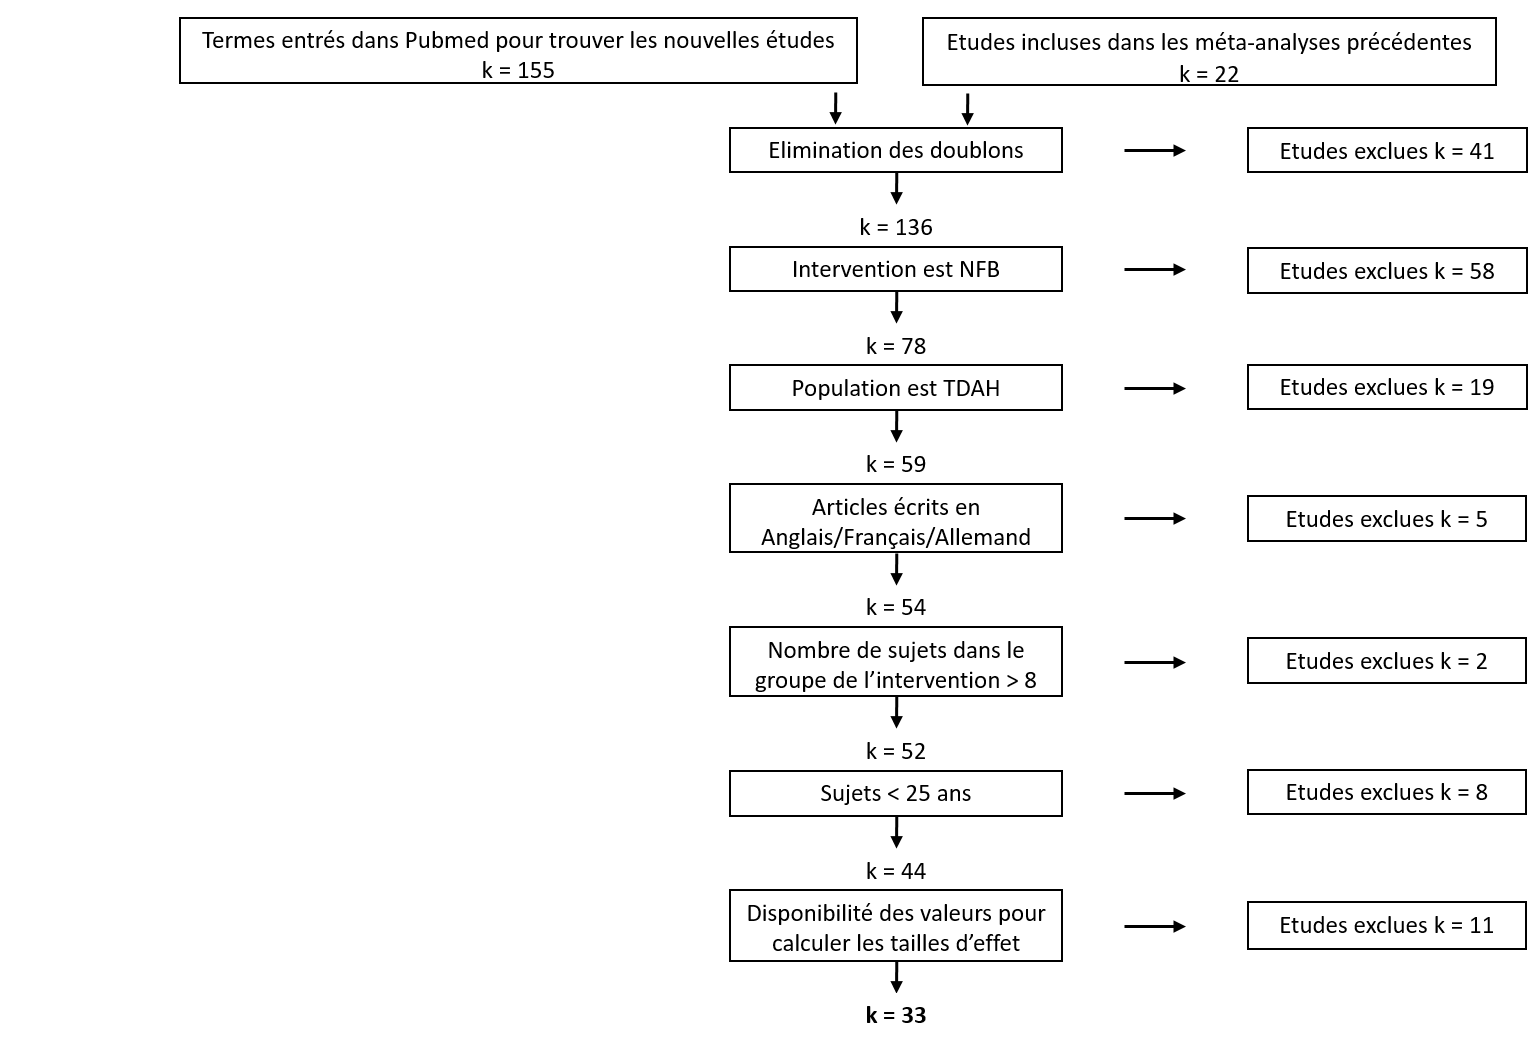
\includegraphics[width=1\linewidth]{figures/chapter-3/factors-selection-studies} 
  \caption[Diagramme de sélection des études pour l'analyse systématique des biais.]{Diagramme de sélection des études pour l'analyse systématique des biais (dernière recherche le 2 septembre 2019).} 
  \label{Figure:factors_pipeline_selection_studies}
\end{figure}

Les \gls{es}-intra-groupe sont calculés pour chaque étude puis les valeurs aberrantes sont rejetées comme expliqué en \ref{es_within}. 
La distribution des \gls{es}-intra-groupe ainsi que les bornes de l'intervalle d'inclusion sont représentées à la 
Figure~\ref{Figure:distribution_ES_within}. Les \gls{es}-intra-groupe négatifs sont en faveur du \gls{nfb}.

\begin{figure}[h!]
  \centering
	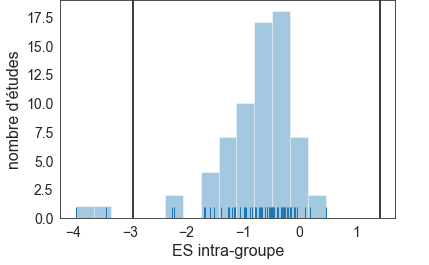
\includegraphics[width=0.7\linewidth]{figures/chapter-3/distribution-ES-within} 
  \caption[Distribution des tailles d'effet intra-groupe calculées pour les études incluses dans la \gls{saob}.]{Distribution des tailles d'effet (\gls{es}) intra-groupe calculées pour les études 
	incluses dans la \gls{saob}, une valeur négative est en faveur du Neurofeedback. Les lignes 
	verticales noires correspondent aux bornes supérieure et 
	inférieure de l'intervalle dans lequel les observations sont acceptées. La courbe verte est la Gaussienne ayant pour paramètres $\mu =$ la moyenne
	de tous les \gls{es} intra-groupe et $\sigma =$ l'écart-type calculé sur tous les \gls{es} intra-groupe}
  \label{Figure:distribution_ES_within}
\end{figure}

Sur la base de notre critère d'exclusion défini en \ref{preprocessing}, $i = 3$ observations (3.40\% du nombre total d'observations) issues de deux études (4.87\% du nombre total d'études) 
sont rejetées : deux groupes de sujets de \citet{Bazanova2018} (celui de l'individualisation du \gls{nfb} et 
celui de l'individualisation du \gls{nfb} et du couplage avec \gls{emg}-Biofeedback) et les résultats obtenus avec les évaluations des 
parents de \citet{Rajabi2019}. 

En effet, ces trois observations présentent des \gls{es}-intra-groupe très larges, notamment les groupes de \citet{Bazanova2018} 
(respectivement -3.41 et -3.95). Ces \gls{es} extrêmement surprenants sont même plus élevés que ceux rapportés dans la littérature sur l'efficacité 
des psychostimulants sur les symptômes du \gls{tdah} chez les enfants \citep{Luan2017} comme illustré à la Figure~\ref{Figure:introduction-efficacy-treatments}. 
Ces valeurs invalident nos hypothèses de travail : dans le cas de la 
\gls{wls}, les résidus ne sont plus distribués normalement. Ainsi, afin de pouvoir conclure sur les résultats obtenus par la \gls{saob}, 
un rejet des valeurs aberrantes a été implémenté.

La \gls{saob} est donc effectuée sur 41 études (qui correspondent à 85 observations) évaluant l'efficacité du \gls{nfb} sur les enfants \gls{tdah} et 
qui sont listées dans la Table~\ref{Table:table_factors_analysis_meta_analysis_list_studies}. Au total, les 41 études sélectionnées rassemblent 
1 153 enfants \gls{tdah} effectuant du \gls{nfb}.

\newpage\
\begin{table}[h!]
  \centering
  \caption[Liste des études incluses dans l'analyse systématique des biais.]{Liste des études incluses dans l'analyse systématique des biais : a) études incluses dans \citet{Cortese2016}
	(dernière recherche le 30 août 2015) ; b) études satisfaisant le critère d'inclusion de \citet{Cortese2016} (dernière recherche le 2 septembre 2019) ; c) études 
	satisfaisant le critère d'inclusion de \citet{Cortese2016} à l'exception de la partie concernant le groupe contrôle (dernière recherche le 2 septembre 2019).}
  \fontsize{9}{11}\selectfont
\begin{tabular}{ cccccc }
\toprule
\multicolumn{3}{ c }{Analyse} & Etude & Année & \shortstack{ Nombre de sujets \\ dans le groupe \\ \gls{nfb} } \\
\midrule
 & & & \citeauthor{Arnold2014} & 2014 & 26 \\ 
 & & & \citeauthor{Bakhshayesh2011} & 2011 & 18 \\
 & & & \citeauthor{Beauregard2006} & 2006 & 15 \\
 & & & \citeauthor{Bink2014} & 2014 & 45 \\
 & & & \citeauthor{Christiansen2014} & 2014 & 14 \\
 & & & \citeauthor{Gevensleben2009} & 2009 & 59 \\
 & & & \citeauthor{Heinrich2004} & 2004 & 13 \\
 & & & \citeauthor{Holtmann2009} & 2009 & 20 \\
 & & & \citeauthor{Linden1996} & 1996 & 9 \\
 & & & \citeauthor{Maurizio2014} & 2014 & 13 \\
 & & & \citeauthor{Steiner2011} & 2011 & 9 \\
 & & & \citeauthor{Steiner2014} & 2014 & 34 \\
 & & & \citeauthor{VanDongen2013} & 2013 & 22 \\
 & & \shortstack{a = Réplication de \\ \citeauthor{Cortese2016}  \\ (voir \ref{replication}) } & \textbf{13 études} & & \textbf{297} \\
\cmidrule(lr){3-6}
 & & & \citeauthor{Aggensteiner2019} & 2019 & 75 \\
 & & & \citeauthor{Baumeister2016} & 2016 & 8 \\
 & & & \citeauthor{Bazanova2018} & 2018 & 17 \\
 & & & \citeauthor{Minder2018} & 2018 & 38 \\
 & & & \citeauthor{Moreno2019} & 2019 & 19 \\
 & & & \citeauthor{Strehl2017} & 2017 & 72 \\
 & & & \citeauthor{Shereena2019} & 2019 & 15 \\
 & \shortstack{b = Mise à jour \\ \citeauthor{Cortese2016} \\ (voir \ref{selection_studies}) } & & \textbf{16 études} & & \textbf{541} \\
\cmidrule(lr){2-6}
 & & & \citeauthor{Bluschke2016} & 2016 & 19 \\
 & & & \citeauthor{Cueli2019} & 2019 & 64 \\
 & & & \citeauthor{Deilami2016} & 2016 & 12 \\
 & & & \citeauthor{Drechsler2007} & 2007 & 17 \\
 & & & \citeauthor{Duric2012} & 2012 & 23 \\
 & & & \citeauthor{Escolano2014} & 2014 & 20 \\
 & & & \citeauthor{Fuchs2003} & 2003 & 22 \\
 & & & \citeauthor{Gelade2016} & 2016 & 39 \\
 & & & \citeauthor{Heinrich2019} & 2019 & 60 \\
 & & & \citeauthor{Kropotov2005} & 2005 & 86 \\
 & & & \citeauthor{Lee2017} & 2017 & 18 \\
 & & & \citeauthor{Leins2007} & 2007 & 19 \\
 & & & \citeauthor{Li2013} & 2013 & 32 \\
 & & & \citeauthor{Meisel2014} & 2014 & 12 \\
 & & & \citeauthor{Mohagheghi2017} & 2017 & 30 \\
 & & & \citeauthor{Mohammadi2015} & 2015 & 16 \\
 & & & \citeauthor{Monastra2002} & 2002 & 51 \\
 & & & \citeauthor{Ogrim2013} & 2013 & 13 \\
 & & & \citeauthor{Rajabi2019} & 2019 & 16 \\
 & & & \citeauthor{Sudnawa2018} & 2018 & 20 \\
 & & & \citeauthor{Strehl2006} & 2006 & 23 \\
 c = \gls{saob} & & & \textbf{41 études} & & \textbf{1 153} \\
\bottomrule
\end{tabular}

  \label{Table:table_factors_analysis_meta_analysis_list_studies}
\end{table}

\newpage\
\subsection{Facteurs identifiés méthode par méthode}

Vingt-huit paramètres ont été initialement identifiés afin d'analyser leur influence sur l'efficacité du \gls{nfb}. Parmi eux, dix ont dû être exclus car ils étaient trop
homogènes ou présentaient trop d'observations manquantes sur la base des critères présentés en \ref{preprocessing} : 
\begin{itemize}
	\item le protocole visant l'augmentation du rythme beta dans les aires frontales,
	\item la présence d'un \gls{irb},
  \item l'utilisation d'une carte pour le transfert de ce qui a été appris durant l'entrainement à la maison et à l'école, 
  \item le type de seuillage pour les récompenses discrètes (incrémental ou fixe),
  \item la qualité de l'acquisition de l'\gls{eeg} égale à 3,
	\item la présence d'un groupe contrôle,
	\item l'individualisation des bandes de fréquences basée sur la valeur de l'\gls{iapf},
	\item le couplage entre le \gls{nfb} et l'\gls{emg}-Biofeedback qui demande au sujet de contrôler son activité cérébrale ene même temps que musculaire,
	\item la sévérité des symptômes du \gls{tdah},
	\item le degré d'engagement dans l'entraînement par \gls{nfb}.
\end{itemize} 

Afin de mettre en évidence la variabilité des valeurs au sein des facteurs non-catégoriels sélectionnés, les \textit{boxplots} des valeurs standardisées ont 
été obtenus et représentés à la Figure~\ref{Figure:factors-boxplots} :
\begin{figure}[h!]
  \centering
	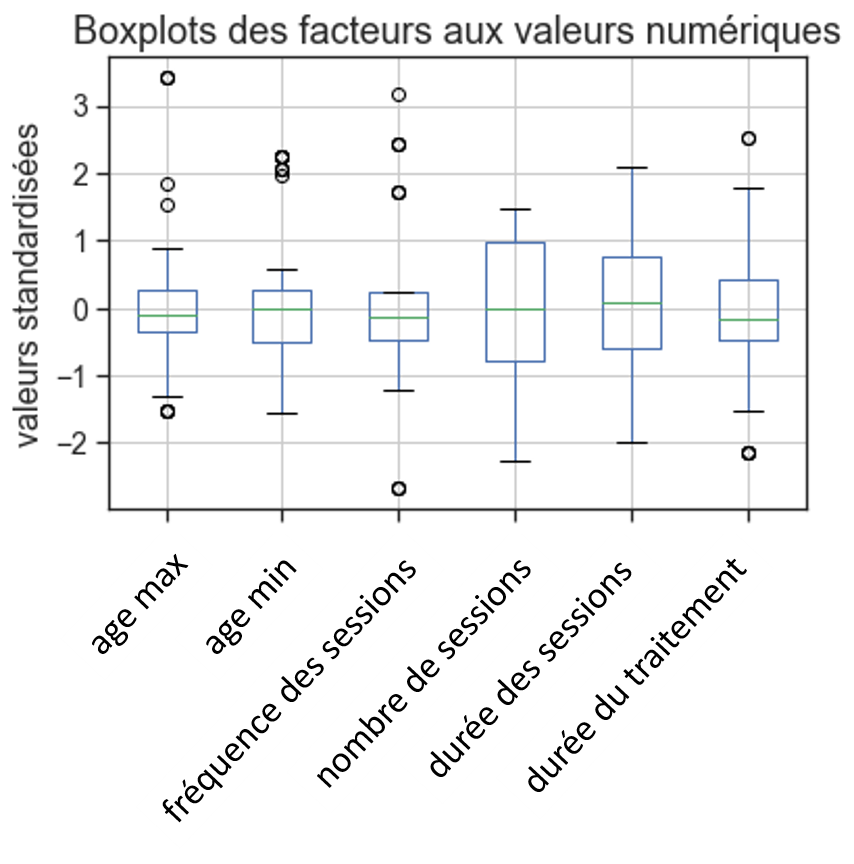
\includegraphics[width=0.7\linewidth]{figures/chapter-3/factors-distribution-of-factors} 
  \caption[\textit{Boxplots} des facteurs aux valeurs numériques standardisées.]{\textit{Boxplots} des facteurs aux valeurs numériques standardisées.} 
  \label{Figure:factors-boxplots}
\end{figure}

Le nombre de sessions et la durée de la session sont plus variables que l'âge minimal et maximal des enfants inclus dans une étude. 

Les trois méthodes décrites précédemment sont donc appliquées tour à tour sur les dix-huit facteurs restants. Tous les résultats sont résumés dans la 
Table~\ref{Table:table_factors_analysis_results_summary}.

\newpage\
\begin{table}[h!]
  \centering
  \caption[Resultats de l'analyse systématique des biais.]{Resultats de la régression linéaire pondérée (\gls{wls}), de la régression linéaire régularisée (\gls{lasso}) et de l'arbre de décision (\gls{dt}). Pour la \gls{wls}, une $p$-value $<$ 0.05 
	(en gras) signifie que le coefficient du facteur correspondant est significativement différent de 0. Pour le \gls{lasso}, les facteurs dont les coefficients sont non mis à 0 (en gras) sont 
	sélectionnés. Pour l'arbre de décision, la place du facteur dans l'arbre est indiquée. Pour les deux premières colonnes, quand la valeur du coefficient est négative le facteur 
	correspondant pourrait mener à de meilleurs résultats du \gls{nfb}.}
  \begin{center}
\small 
\begin{tabular}{ p{3cm} p{3cm} p{3cm} p{2cm} p{2cm} p{2cm}}
\toprule
\multicolumn{2}{c}{ \shortstack{Variables \\ indépendantes (facteurs)} } & \shortstack{ Coefficients \\ trouvés par \gls{wls} \\ ($p$-value) } & \shortstack{ Coefficients \\ trouvés par \\ \gls{lasso} } & \shortstack{Place \\ sur le \\ \gls{dt}} \\
\midrule
\multirow{ 3}{*}{ \textit{Méthodologiques} } & \gls{pblind} & \hskip 0.12in\textbf{0.15 (0.015)} & \hskip 0.12in\textbf{0.086} & \textbf{\textit{root node}} \\ 
& randomisation & \hskip 0.12in0.013 (0.840) & \hskip 0.12in0.00 & / \\   
\midrule
\multirow{ 3}{*}{ \textit{Population} } & age max & \hskip 0.08in-0.10 (0.106) & \hskip 0.12in0.00 & / \\
& age min & \hskip 0.12in0.056 (0.43) & \hskip 0.12in0.00 & / \\
& prise de médicaments & \hskip 0.08in-0.026 (0.72) & \hskip 0.12in0.00 & / \\
\midrule
\multirow{ 9}{*}{ \textit{ \shortstack{Implementation \\ du \gls{nfb}} } } & nombre de sessions & \hskip 0.08in\textbf{-0.19 (0.025)} & \hskip 0.12in0.00 & / \\
& durée de la session & \hskip 0.08in-0.13 (0.16) & \hskip 0.12in0.00 & \textbf{2$^{eme}$ noeud} \\
& durée du traitement & \hskip 0.12in\textbf{0.39 (0.00)} & \hskip 0.12in\textbf{0.098} & \textbf{2$^{eme}$ et 3$^{eme}$ noeuds} \\
& fréquence des sessions & \hskip 0.12in0.027 (0.690) & \hskip 0.08in\textbf{-0.055} & \textbf{2$^{eme}$ noeud} \\ 
& \gls{smr} & \hskip 0.12in0.12 (0.067) & \hskip 0.12in0.00 & / \\
& augmentation de beta en central & \hskip 0.12in0.087 (0.32) & \hskip 0.12in\textbf{0.026} & / \\  
& diminution de theta & \hskip 0.08in-0.095 (0.39) & \hskip 0.12in0.00 & / \\
& \gls{scp} & \hskip 0.08in-0.14 (0.30) & \hskip 0.12in0.00 & / \\ 
& phase de transfert & \hskip 0.12in\textbf{0.33 (0.001)} & \hskip 0.12in\textbf{0.079} & \textbf{1$^{er}$ noeud} \\
\midrule
\multirow{ 2}{*}{ \textit{ \shortstack{Qualité de \\ l'acquisition} } } & plus d'une électrode d'enregistrement & \hskip 0.08in-0.083 (0.20) & \hskip 0.08in\textbf{-0.030} & / \\ 
& \gls{eeg} qualité 2 & \hskip 0.08in\textbf{-0.28 (0.00)} & \hskip 0.08in\textbf{-0.037} & / \\  
\midrule
\multirow{ 2}{*}{ \textit{Qualité du signal} } & rejet ou correction des artefacts oculaires & \hskip 0.08in-0.10 (0.164) & \hskip 0.08in\textbf{-0.0046} & \textbf{1$^{er}$ noeud} \\ 
& rejet des artefacts basé sur l'amplitude & \hskip 0.12in0.14 (0.058) & \hskip 0.12in0.00 & / \\   
\bottomrule
\end{tabular}
\end{center}

  \label{Table:table_factors_analysis_results_summary}
\end{table}

\subsubsection{La régression linéaire multiple et pondérée}

Les hypothèses de ce modèle sont respectées, les résultats sont interprétables :
\begin{itemize}
	\item la matrice ${\textbf{X}}^{T}\textbf{W}^{T}\textbf{WX}$ est bien régulière,
  \item la tendance linéaire estimée est trouvée significative (Prob(F-statistic) = 1.56e-05),
  \item les résidus sont distribués normalement (Kurtosis = 4.15, \textit{Skewness} = -0.29 et Prob(Omnibus) = 0.055).
\end{itemize}

La \gls{wls} a trouvé 5 facteurs significatifs (deuxième colonne de la Table~\ref{Table:table_factors_analysis_results_summary}) avec un \textit{adjusted R Squared} de 0.39. 
Dans le cas de l'\gls{ols}, les mêmes facteurs ont été trouvés significatifs (à l'exception du nombre de sessions) mais avec un \textit{adjusted R Squared} plus faible (0.20). Ainsi, associer un poids
à chaque observation permet d'expliquer davantage de variabilité. 

Il est important de noter qu'étant donné qu'un \gls{es}-intra-groupe négatif est en faveur de l'efficacité du \gls{nfb},
un facteur dont le coefficient est négatif aurait une influence positive sur les résultats \gls{nfb}.


\subsubsection{La régression linéaire régularisée}

La validation croisée \textit{leave-one-out} illustrée à la Figure~\ref{Figure:selection_lambda_lasso} a permis de déterminer un $\lambda$ optimal égal à 0.039.
\begin{figure}[h!]
  \centering
	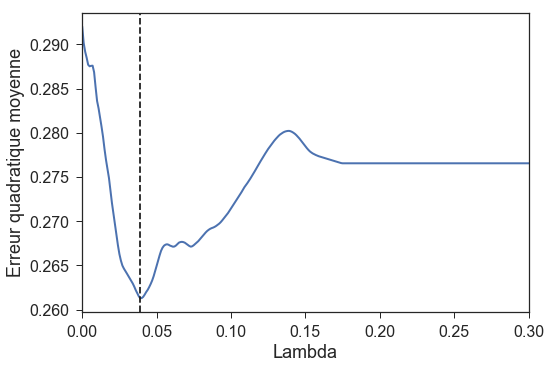
\includegraphics[width=0.7\linewidth]{figures/chapter-3/factors-selection-lasso-best-lambda} 
  \caption[Erreur quadratique moyenne obtenue sur la moyenne de tous les \textit{folds} utilisés lors de la validation 
	croisée \textit{leave-one-out}.]{Erreur quadratique moyenne (\gls{mse}) obtenue sur la moyenne de tous les \textit{folds} utilisés lors de la validation 
	croisée \textit{leave-one-out}. La courbe bleue représente la \gls{mse} moyennée sur tous les \textit{folds} ; la droite verticale en pointillés correspond
	au minimum de la \gls{mse} moyenne.}
  \label{Figure:selection_lambda_lasso}
\end{figure}

Le \gls{lasso} a gardé huit facteurs différents de 0 (troisième colonne de la Table~\ref{Table:table_factors_analysis_results_summary}). Pour cette méthode également,
un facteur dont le coefficient est négatif aurait un bon impact sur l'efficacité du \gls{nfb}.

\subsubsection{L'arbre de décision de régression}

L'arbre de décision obtenu est présenté à la Figure~\ref{Figure:factors_decision_tree} : \gls{pblind} est le meilleur prédicteur (dernière colonne de la
Table~\ref{Table:table_factors_analysis_results_summary}). Cinq autres facteurs divisent ensuite les sous-ensembles, toutefois étant donné que de moins
en moins d'observations sont disponibles plus on descend dans l'arbre, l'influence de ces facteurs est de moins en moins certaine.

\begin{figure}[h!]
  \centering
	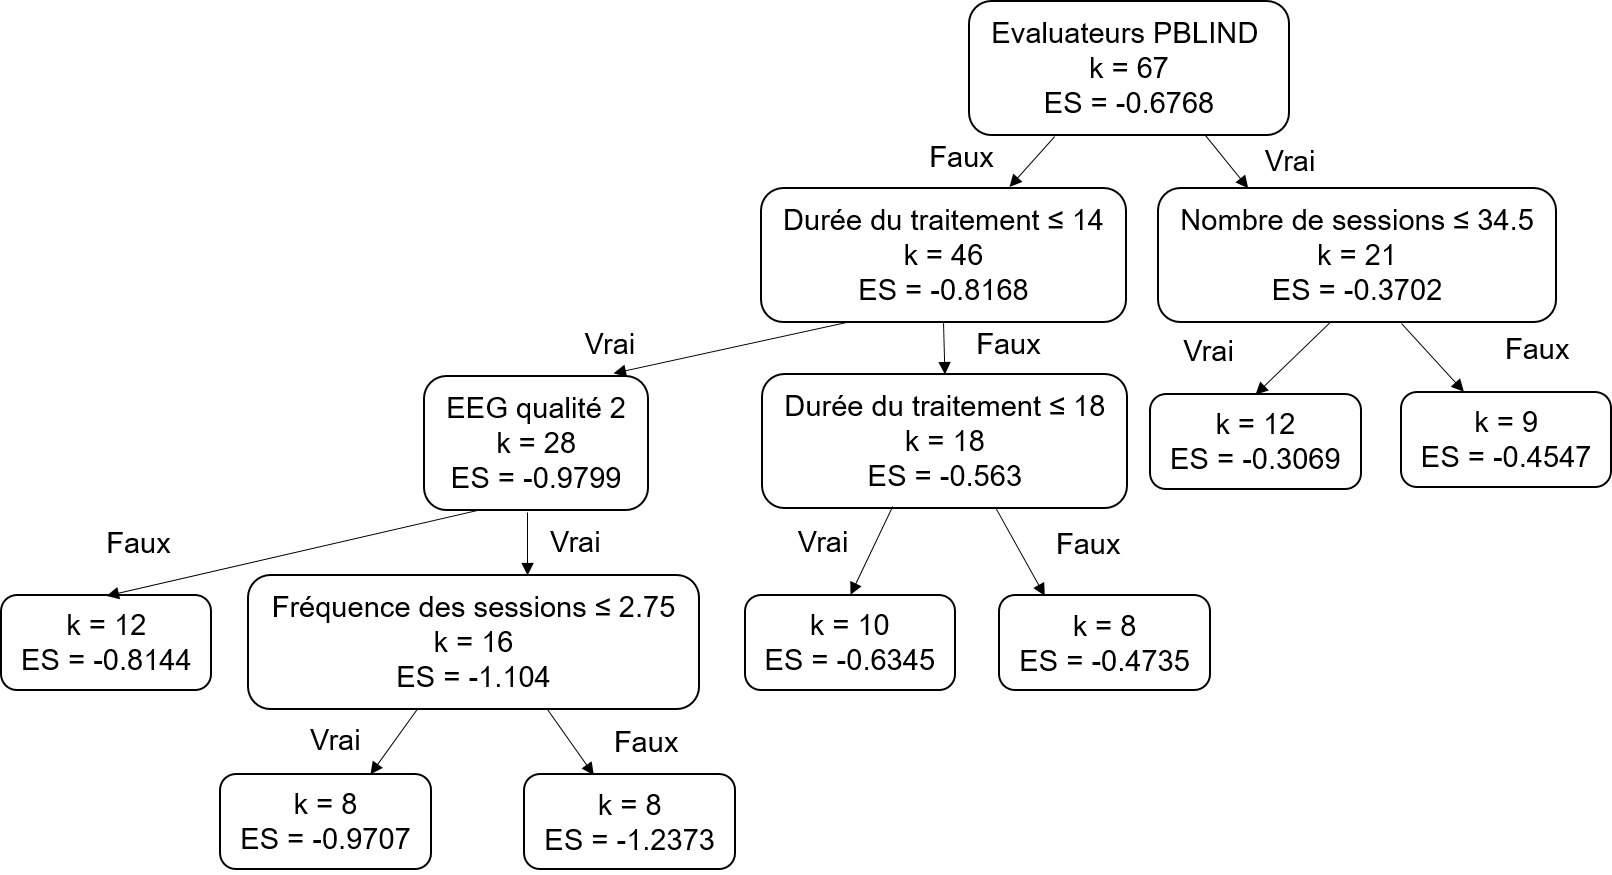
\includegraphics[width=1\linewidth]{figures/chapter-3/factors-decision-tree} 
  \caption[Arbre de décision]{Arbre de décision obtenu : \gls{es} correspond à l'\gls{es}-intra-groupe et $k$ au nombre d'études. L'importance des variables indépendantes
	décroît depuis le \textit{root node}. La durée de la session est mesurée en minutes et la durée du traitement en semaines.}
  \label{Figure:factors_decision_tree}
\end{figure}

\subsection{Résumé des résultats}

Plusieurs facteurs ont été trouvés significatifs par les trois méthodes : les évaluateurs \gls{pblind}, la durée du traitement et la présence d'une phase de transfert. 
De plus, toutes les méthodes s'accordent quant à la direction de leur influence : alors qu'évaluer l'efficacité du \gls{nfb} en étant \gls{pblind}
et intégrer une phase de transfert dans l'entrainement semblent conduire à de moins bons résultats, une durée de traitement plus courte mènerait à un traitement plus efficace. 

L'influence des facteurs retournés par deux méthodes est plus incertaine :
\begin{itemize}
	\item la \gls{wls} et le \gls{lasso} trouvent tous deux qu'une bonne qualité d'acquisition est préférable,
  \item le \gls{lasso} et le \gls{dt} obtiennent tous deux qu'un nombre élevé de sessions par semaine et que la correction ou le rejet des artefacts oculaires
	influenceraient positivement les résultats. 
\end{itemize}

Quatre facteurs sont retournés seulement par une méthode : le nombre de sessions, l'augmentation du rythme beta dans la zone centrale, l'enregistrement
de l'\gls{eeg} par plus d'une électrode et la durée de la session. 

Huit facteurs, n'ont quant à eux été sélectionnés par aucune méthode : la randomisation des sujets, l'âge minimum et maximum des enfants, prendre des 
médicaments pendant le traitement par \gls{nfb}, les protocoles \gls{smr}, diminution de theta et \gls{scp}, et le rejet
des artefacts basée sur l'amplitude. Ainsi ces facteurs n'influenceraient pas l'efficacité du \gls{nfb}. 

Ces résultats sont résumés à la Table~\ref{Table:table_factors_analysis_results_summary_number_of_factors}.

\begin{table}[h!]
  \centering
  \caption[Facteurs classés selon le nombre de méthodes les identifiant comme significatifs.]{Facteurs classés selon le nombre de méthodes les identifiant comme significatifs. Un signe + signifie que la présence (dans le cas d'une variable catégorielle) ou l'importante valeur
	de la variable a un effet favorable sur l'efficacité du \gls{nfb}. A l'inverse, un signe - signifie que l'absence (dans le cas d'une variable catégorielle) ou la faible valeur
	de la variable a un effet favorable sur l'efficacité du \gls{nfb}. Le nombre de signes est décroissant avec le degré de confiance accordé à l'influence du facteur. 0 signifie 
	que le facteur n'aurait pas d'effet.}
  \begin{center}
\small 
\begin{tabular}{ ccc }
\toprule
\shortstack{Nombre de \\ méthodes}  & Facteurs & \shortstack{ Sens de \\ l'influence } \\
\midrule
\multirow{ 3}{*}{ \textit{3 méthodes} } & \gls{pblind} & - - - \\ 
& durée du traitement & - - - \\  
& phase de transfert & - - - \\  
\midrule
\multirow{ 3}{*}{ \textit{2 méthodes} } & \gls{eeg} qualité 2 & + + \\
& fréquence des sessions & + + \\
& \gls{eog} rejet ou correction & + + \\
\midrule
\multirow{ 5}{*}{ \textit{1 méthode} } & nombre de sessions & + \\
& durée de la session & - \\
& augmentation de beta en central & - \\
& plus d'une électrode d'enregistrement & + \\
\midrule
\multirow{ 8}{*}{ \textit{ Aucune méthode } } & randomisation & 0 \\ 
& age min & 0 \\ 
& age max & 0\\  
& prise de médicaments & 0 \\
& \gls{smr} & 0 \\
& diminution de theta & 0 \\
& \gls{scp} & 0 \\
& rejet des artefacts basé sur l'amplitude & 0 \\
\bottomrule
\end{tabular}
\end{center}
  \label{Table:table_factors_analysis_results_summary_number_of_factors}
\end{table}

\section{Discussion}

La description et l'analyse des différents types d'implémentation de \gls{nfb} ont fait l'objet de plusieurs études \citep{Arns2014, 
Jeunet2018, Arns2009, Cortese2016, Alkoby2017, Rogala2016, Enriquez2017}. Cependant, à notre connaissance, aucune de ces études n'a implémenté une approche systématique et 
multivariée pour associer les facteurs aux résultats cliniques. 

Toutefois, cette méthode souffre de quelques limitations, comme 
l'utilisation de seulement trois méthodes et le choix de critères arbitraires pour exclure des facteurs et des observations. Par ailleurs, le fait que pour une étude il peut y 
avoir plusieurs observations n'est capturé que par la \gls{wls}. Ensuite, la \gls{saob} ne permet pas de donner de chiffres précis quant à la durée du traitement ou au 
nombre de sessions par exemple : elle permet seulement de conseiller une direction mais sans quantification.

La rigueur et la transparence lors de la conduite d'essais cliniques sur l'efficacité
du \gls{nfb} est essentielle pour comprendre son effet sur les fonctions cérébrales et le comportement comme le soulignent \citet{Ros2019} lors de l'élaboration
de leur liste de bonnes pratiques. Ce point a également été souligné par \citet{Rogala2016} : les méthodologies suivies dans la recherche sur l'efficacité du
\gls{nfb} sont rarement fiables et trop souvent contradictoires.

\subsection{Facteurs et efficacité du \gls{nfb}} \label{discussion_factors}

La \gls{saob} a permis d'identifier des facteurs ayant une potentielle influence sur l'efficacité du \gls{nfb}. Ces facteurs ont été choisis sur la base d'avis d'experts
du \gls{nfb} et de la littérature scientifique sur le sujet. Les résultats trouvés par la \gls{saob} sont discutés ici et mis en perspective avec cette littérature, en s'intéressant à la fois 
aux paramètres pour lesquels l'influence sur la performance clinique est fortement probable et à ceux pour lesquels l'impact s'avère moins certain. 

Tout d'abord, Le type de protocole \gls{nfb} n'a été identifié, étonnamment, par aucune méthode à l'exception de l'augmentation du rythme beta en central qui l'a été par une méthode. 
Ainsi, selon la \gls{saob}, quel que serait le protocole d'entrainement, il n'influencerait pas l'efficacité du \gls{nfb}, son effet serait non-spécifique. Cette importance 
minime octroyée par la \gls{saob} à ces facteurs est contre-intuitive étant donné le rôle central du protocole choisi sur le mode d'action neurophysiologique 
et donc sur l'impact sur l'efficacité thérapeutique \citep{Vernon2004, Heinrich2019}. Une probable 
explication pour ce résultat est que tous ces protocoles ont une efficacité équivalente sur les populations étudiées et donc ne représentent 
pas un facteur explicatif significatif.
  
Un des paramètres souvent étudié est le nombre de sessions qu'il faut effectuer durant le traitement par \gls{nfb}. Dans la plupart des cas, le nombre 
de sessions est fixe et donc défini à l'avance grâce aux résultats obtenus par des études d'efficacité similaires \citep{Enriquez2017}. Cependant malgré le soin apporté
au choix du nombre de sessions, celui-ci n'aurait pas d'influence sur l'efficacité du \gls{nfb} selon la \gls{saob} : il est identifié seulement par la \gls{wls} pour laquelle effectuer 
plus de sessions serait favorable. 

\citet{Vernon2004} a suggéré qu'au moins 20 sessions étaient nécessaires pour observer un effet thérapeutique, 
ce qui a été confirmé par \citet{Arns2014, Arns2009, Wang2014}. 
\citet{Wang2014} a montré sur des enfants sains une amélioration significative de la mémoire de travail suite à 20 sessions d'entrainement cognitif.
Quant à \citet{Arns2009}, plusieurs régressions linéaires sans correction pour tests multiples ont montré une
corrélation positive entre le nombre de sessions et les \gls{es}-intra-groupe pour la composante inattention seulement. 

Le fait que le nombre de sessions n'a pas été identifié par la \gls{wls}
pourrait s'expliquer par la présence de seulement neuf observations de 20 sessions ou moins (ce qui correspond à 7.65\% du nombre total d'observations). 
Ainsi, étant donné que le seuil minimal pour obtenir des résultats avec l'entrainement par \gls{nfb} semble dépassé pour la très grande majorité des observations, 
il est peu probable que ce facteur puisse être retrouvé par les trois méthodes sur cet ensemble de données. 

\citet{Cortese2016} a conduit une méta-régression pour estimer l'influence du nombre de sessions
sur les \gls{es}-inter-groupes calculés sur la composante totale d'une part pour les évaluations des parents et d'autre part pour celles des enseignants : 
dans chacun de ces cas la $p$-value associée à la variable indépendante "nombre de sessions" n'était pas significativement différente de 0, ce qui va dans le sens 
du résultat de la \gls{saob}. Ainsi, il semblerait que d'autres analyses soient nécessaires pour pouvoir trancher sur la réelle influence du nombre de sessions 
et sur son nombre optimal pour favoriser l'efficacité du \gls{nfb}.

Cette notion du nombre de sessions comprend plusieurs aspects comme l'ont souligné \citet{Strehl2014} parmi lesquels la durée du traitement et la fréquence des 
sessions. Afin de se rendre compte du lien entre ces trois paramètres un \textit{pairplot} a été tracé à la Figure~\ref{Figure:factors_pairplot}.

\begin{figure}[h!]
  \centering
	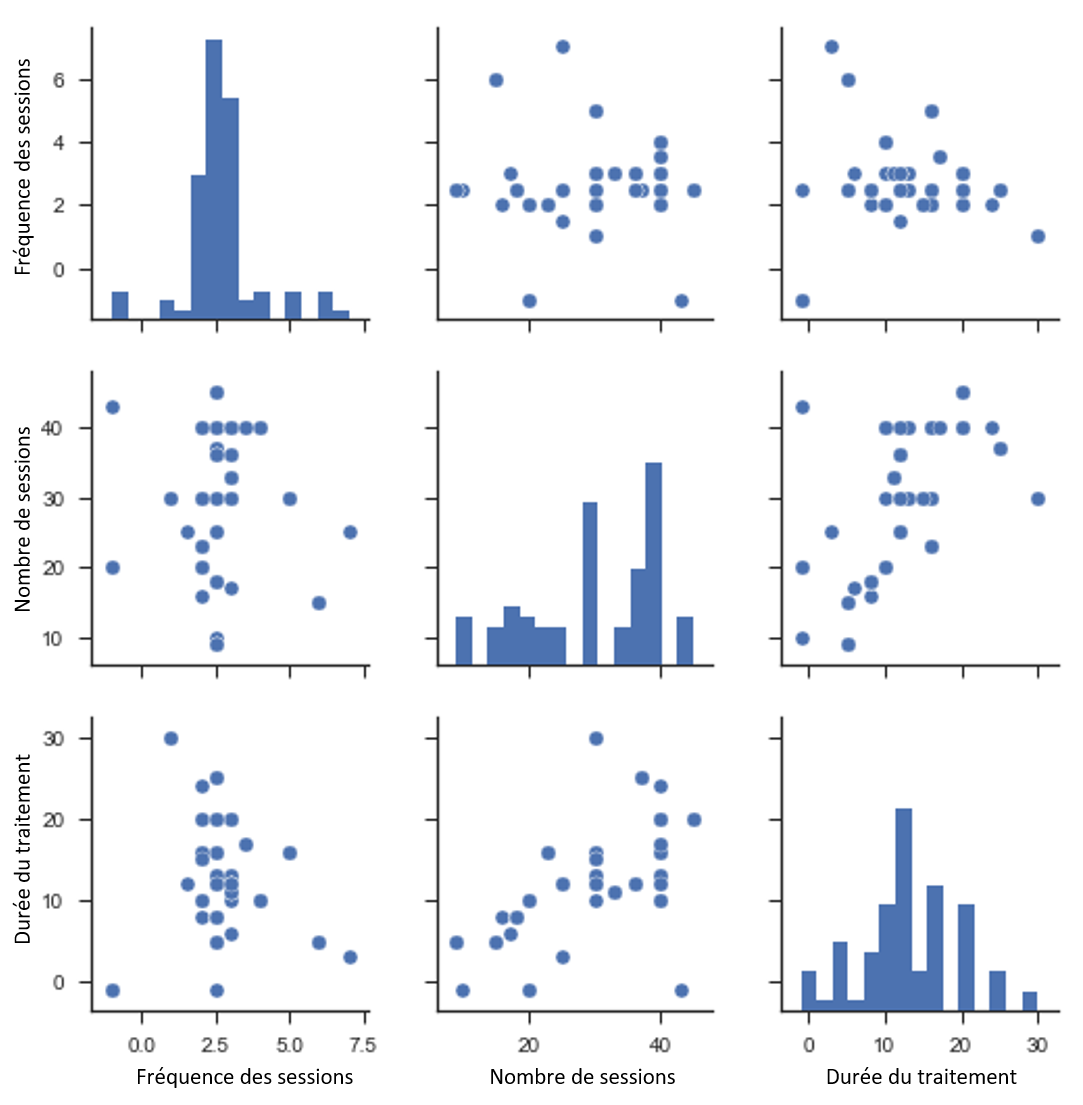
\includegraphics[width=1\linewidth]{figures/chapter-3/factors-pairplot} 
  \caption[\textit{Pairplot} obtenu sur les variables indépendantes non standardisées.]{\textit{Pairplot} obtenu sur les variables indépendantes non standardisées "fréquence des sessions", "nombre de sessions" et "durée du traitement" 
	comprenant les 85 observations retenues suite au prétraitement des données expliqué en \ref{preprocessing}. La fréquence des sessions 
	est donnée en nombre de sessions par semaine et la durée du traitement en semaines.}
  \label{Figure:factors_pairplot}
\end{figure}

Sur ce \textit{pairplot} on peut observer que le nombre de sessions a tendance à augmenter avec la durée du traitement. Par contre, 
la fréquence des sessions reste globalement stable avec l'augmentation du nombre de sessions et la durée du traitement. 

Le facteur "durée du traitement" a justement été identifié par les trois méthodes intégrées dans la \gls{saob} : il semblerait que plus le traitement par 
\gls{nfb} est long, moins il devient efficace. Le degré d'engagement 
dans l'intervention pourrait expliquer ce résultat : être engagé dans un traitement long est plus compliqué. Cependant, il est difficile de quantifier ce degré car, 
soit aucun questionnaire n'est rempli par les enfants à ce sujet, soit cette information n'est pas mentionnée. 

Par ailleurs, la durée du traitement est liée à son intensité : le \textit{paiplot} présenté à la Figure~\ref{Figure:factors_pairplot} montre que même si
la fréquence des sessions est assez stable avec la durée du traitement, dans le cas de traitements courts, la fréquence
des sessions est soutenue pour certaines observations ce qui n'est pas le cas pour les traitement longs. Ainsi on peut 
supposer qu'une période de traitement plus courte est préférable du fait de la fréquence plus élevée des sessions. 

Cette hypothèse est étayée par le fait que la variable "fréquence des sessions" est aussi associée à de plus grands \gls{es}-intra-groupe selon le
\gls{lasso} et le \gls{dt}. L'impact de l'intensité du traitement par \gls{nfb} a été exploré par \citet{Rogala2016} sur des sujets adultes sains : il a été
observé que les études proposant au moins 4 sessions de \gls{nfb} sur des jours consécutifs sont toutes bénéfiques. Toutefois,
\citet{Arnold2014} n'ont noté aucune différence d'amélioration thérapeutique entre les enfants \gls{tdah} effectuant deux sessions par semaine
et ceux en effectuant trois. 

Les résultats de la \gls{saob} indiquent donc qu'adopter une fréquence élevée de sessions est préférable, ce qui est peu connu dans le domaine du \gls{nfb}. 
En effet sur la question de l'intensité du traitement, \citet{Strehl2014} s'est appuyé sur les résultats de l'entrainement cognitif d'enfants 
sains pour lesquels il a observé que des sessions dispersées conduisent à une meilleure efficacité \citep{Wang2014}. \citet{Enriquez2017} ont
également rappelé que dans le milieu de l'éducation, les leçons espacées sont plus efficaces mais ont souligné qu'en ce qui concerne le \gls{nfb},
trop peu d'éléments sont disponibles pour conclure quant au bénéfice de l'espacement des sessions.

Tout comme la durée du traitement, deux autres facteurs ont été identifiés par les trois méthodes avec, de plus, la même direction d'influence : la présence d'une phase de transfert, 
et les évaluateurs probablement aveugles au traitement. Ce dernier est discuté en \ref{pblind_anaysis}.

La phase de transfert ayant pour but d'aider à transposer le contrôle appris lors des séances de \gls{nfb} à la vie de tous les jours, on pourrait donc s'attendre à un effet positif sur les symptômes
du \gls{tdah} comme l'ont avancé \citet{Arns2014, Strehl2006, Gani2008}, or la \gls{saob} conclut à un impact négatif. Ce résultat s'expliquerait peut-être par le fait qu'une phase de 
transfert seule ne soit pas si efficace si elle n'est pas couplée à l'utilisation d'une carte représentant la métaphore utilisée lors des sessions de \gls{nfb} qui permet à l'enfant de se 
souvenir plus facilement du contrôle qu'il exerçait durant la séance \citep{Bioulac2019, Bluschke2016}. Ce facteur devait être analysé mais étant trop homogène (plus de 80\% des observations 
n'utilisent pas de carte), il a été exclus de l'analyse. 

Ce résultat va dans le sens d'un effet purement placebo du \gls{nfb}. Cependant, une mise à jour avec un plus grand nombre de données serait nécessaire pour pouvoir l'affirmer.

Tout comme la fréquence des sessions, deux autres paramètres sont retournés par deux méthodes et donc pourraient influencer 
l'efficacité du \gls{nfb} : la qualité de l'\gls{eeg} égale à 2 et la correction ou rejet des artefacts oculaires.

En effet, selon deux méthodes, enregistrer l'\gls{eeg} dans de bonnes conditions mènerait à de meilleurs résultats. Cette observation peut s'expliquer par le fait qu'un signal
\gls{eeg} de bonne qualité permet l'extraction plus précise des caractéristiques de l'\gls{eeg} liées au \gls{tdah} et donc conduit à un meilleur apprentissage et 
à une efficacité thérapeutique augmentée. Cependant, évaluer la qualité des moyens d'acquisition de l'\gls{eeg} (comme l'amplificateur utilisé) 
est difficile du fait du peu d'informations fourni par les études à ce sujet. Par conséquent, les futures essais cliniques devraient apporter plus 
de précisions quant au matériel utilisé afin de pouvoir plus aisément juger de sa qualité. La qualité d'acquisition de signaux \gls{eeg} peut être évaluée grâce à différentes
métriques dont certaines ont été utilisées par \citep{Bussalb2018benchmark} lors de la comparaison de différents systèmes \gls{eeg}. 

Deux méthodes s'accordent également sur le fait que corriger ou rejeter les artefacts oculaires aurait un impact positif sur l'efficacité du \gls{nfb}. Ce résultat peut également
s'expliquer par le fait qu'un signal \gls{eeg} non contaminé par des artefacts permet d'extraire plus précisément les neuromarqueurs \citep{Barthelemy2017, Barthelemy2019} étant donné l'impact
des mouvements oculaires et clignements sur l'\gls{eeg} souligné en \ref{steps_NFB_taining} \citep{Iwasaki2005}. 

\subsection{Perspectives pour de futures analyses}

L'influence d'autres facteurs sur l'efficacité du \gls{nfb} aurait été intéressante à analyser, comme la personnalisation des 
protocoles d'entrainement basée sur l'\gls{iapf}. En effet, \citet{Vernon2004} et \citet{Klimesch1999} ont noté que les limites des bandes 
de fréquence varient d'un individu à l'autre et sont aussi dépendantes de l'âge. Par ailleurs, les résultats paraissent prometteurs selon 
\citet{Bazanova2018, Escolano2014} et \citet{Alkoby2017}. Cependant, ce paramètre n'a pas pu être inclus dans la \gls{saob} faute d'un 
nombre suffisant d'études proposant un protocole personnalisé. Ce manque d'études est aussi la raison pour laquelle le couplage entre l'\gls{emg}-Biofeedback 
et le \gls{nfb} n'a pas pu être étudié dans la \gls{saob}. 

Un autre facteur intéressant, qui aurait pu aider à expliquer les résultats sur la durée du traitement, a 
également été exclu de l'analyse : la sévérité des symptômes à pré-test. Bien que les scores à pré-test soient disponibles pour chaque étude, ils ne sont pas
comparables car différentes échelles sont utilisées. Afin de résoudre ce problème, ces scores ont été normalisés grâce au score maximum pouvant être atteint
sur chaque échelle. Toutefois, cette valeur n'a pas pu être trouvée pour plusieurs échelles cliniques : trop d'observations manquantes ont mené au rejet du facteur.

Ensuite, il serait intéressant de s'intéresser au lieu où les sessions de \gls{nfb} sont effectuées. En effet, \citet{Minder2018} ont souligné le fait que le lieu
d'entrainement pourrait aussi être un facteur contribuant à l'efficacité du \gls{nfb}. Toutefois, dans leur étude aucune différence significative 
n'est trouvée entre les résultats des performances à la clinique et à l'école. \citet{Vernon2004} a avancé qu'effectuer les séance de \gls{nfb} à l'école
pourrait faciliter le transfert de ce qui a été appris lors des sessions de \gls{nfb} à la vie de tous les jours.

Dans la grande majorité des études sur le \gls{nfb} appliqué aux enfants
\gls{tdah}, les sessions ont lieu en clinique, rendant impossible à la \gls{saob} d'étudier ce facteur. Cependant, à l'instar de \citet{Steiner2014, Minder2018}, 
d'autres études demandent à leurs sujets d'effectuer leurs séances en dehors du milieu hospitalier \citep{Bioulac2019}, ainsi l'influence du lieu d'entrainement 
pourra finir par être étudiée plus précisément. Cela sera aussi valable pour les facteurs évoqués plus tôt et qui ont dû être exclus de la \gls{saob}.

Un paramètre central dans l'entrainement par \gls{nfb} a également été exclu de la \gls{saob} faute d'un nombre suffisant d'études, il s'agit du type de seuillage 
grâce auquel les récompenses sont retournées au sujet. Sa définition est centrale pour l'entrainement par \gls{nfb}, cependant elle varie énormément d'une 
étude à l'autre. En effet, le seuil peut être le même tout au long du traitement ou adaptatif, il peut être fixé manuellement ou automatiquement. 

Le seuil peut être fixe durant le traitement ou bien s'adapter aux performances du sujet au cours de la session ou entre les sessions ce qui semble 
préférable selon \citep{Bauer2016}. Une des raisons évoquées pour utiliser un seuil adaptatif est de garder le sujet motivé en le récompensant de manière régulière 
\citep{Lansbergen2011}. Cependant, cette approche conduit parfois à récompenser le sujet alors que ses performances ne le justifient pas. En effet, comme souligné par \citep{Strehl2014},
dès que le sujet est trop ou trop peu récompensé, le seuil est ajusté, rendant la motivation du sujet plus importante que la qualité de la performance.

Selon \citet{Arns2014}, le seuillage automatique est contraire aux prinicipes de la théorie de l'apprentissage : ce type de seuillage ne récompense
pas le sujet sur ses réelles performances d'auto-régulation. Cependant, adapter manuellement la valeur du seuil contraint le sujet à effectuer ses sessions en 
clinique et empêche la mise en place d'un double aveugle \citep{Lansbergen2011} qui est pourtant recommandé \citep{Ros2019}. 

Enfin, l'influence du type de \textit{feedback} (visuel, auditif, tactile) n'a pas été étudiée ici mais a déjà été discutée dans la littérature, 
notamment par \citet{Vernon2004} qui a avancé que coupler le retour visuel et auditif serait préférable. 

\subsection{Analyse approfondie des évaluateurs probablement aveugles} \label{pblind_anaysis}

Les résultats de la \gls{saob} sont globalement en faveur de l'efficacité du \gls{nfb} pour le traitement des enfants \gls{tdah}, notamment l'utilisation 
de systèmes d'acquisition de bonne qualité et le rythme soutenu du traitement. Toutefois, comme attendu, l'évaluation
des symptômes par des personnes non-aveugles (\gls{mprox}) conduit à des résultats plus favorables que celles des évaluateurs \gls{pblind}, ce qui est en accord avec les
méta-analyses existantes \citep{Micoulaud2014, Cortese2016}. 

Les enseignants sont considérés comme \gls{pblind} par \citet{Cortese2016, Micoulaud2014} et cette définition a été suivie dans la \gls{saob}. Etonnamment, les données
à disposition ne vont pas exactement dans le sens de l'hypothèse largement acceptée que la différence entre \gls{mprox} et \gls{pblind} peut être seulement 
expliquée par l'effet placebo. Par ailleurs, les enseignants sont désignés comme "probablement" aveugles, ce qui signifie qu'ils peuvent être au courant du
traitement suivi par les enfants. En effet, il est possible que certains enseignants voient les enfants prendre des psychostimulants lors des pauses.
Cependant, il est difficile d'évaluer l'amplitude de ce phénomène. 

Un élément corrobore cette hypothèse : pour chaque étude incluse dans cette analyse, l'évaluation des symptômes avant le début
du traitement par les parents comparée à celle des enseignants montre que ces derniers ne voient pas l'ensemble des symptômes, autrement dit qu'ils sont probablement
plus aveugles aux symptômes qu'au traitement comme l'illustre la Figure~\ref{Figure:factors_pblind_discussion}. En effet, à pré-test, les enseignants évaluent les 
symptômes moins sévèrement que les parents et observent moins d'amélioration à post-test : cela correspond davantage au cas \textbf{A} représentant l'absence d'effet placebo
qu'au cas \textbf{B}.

\begin{figure}[h!]
  \centering
	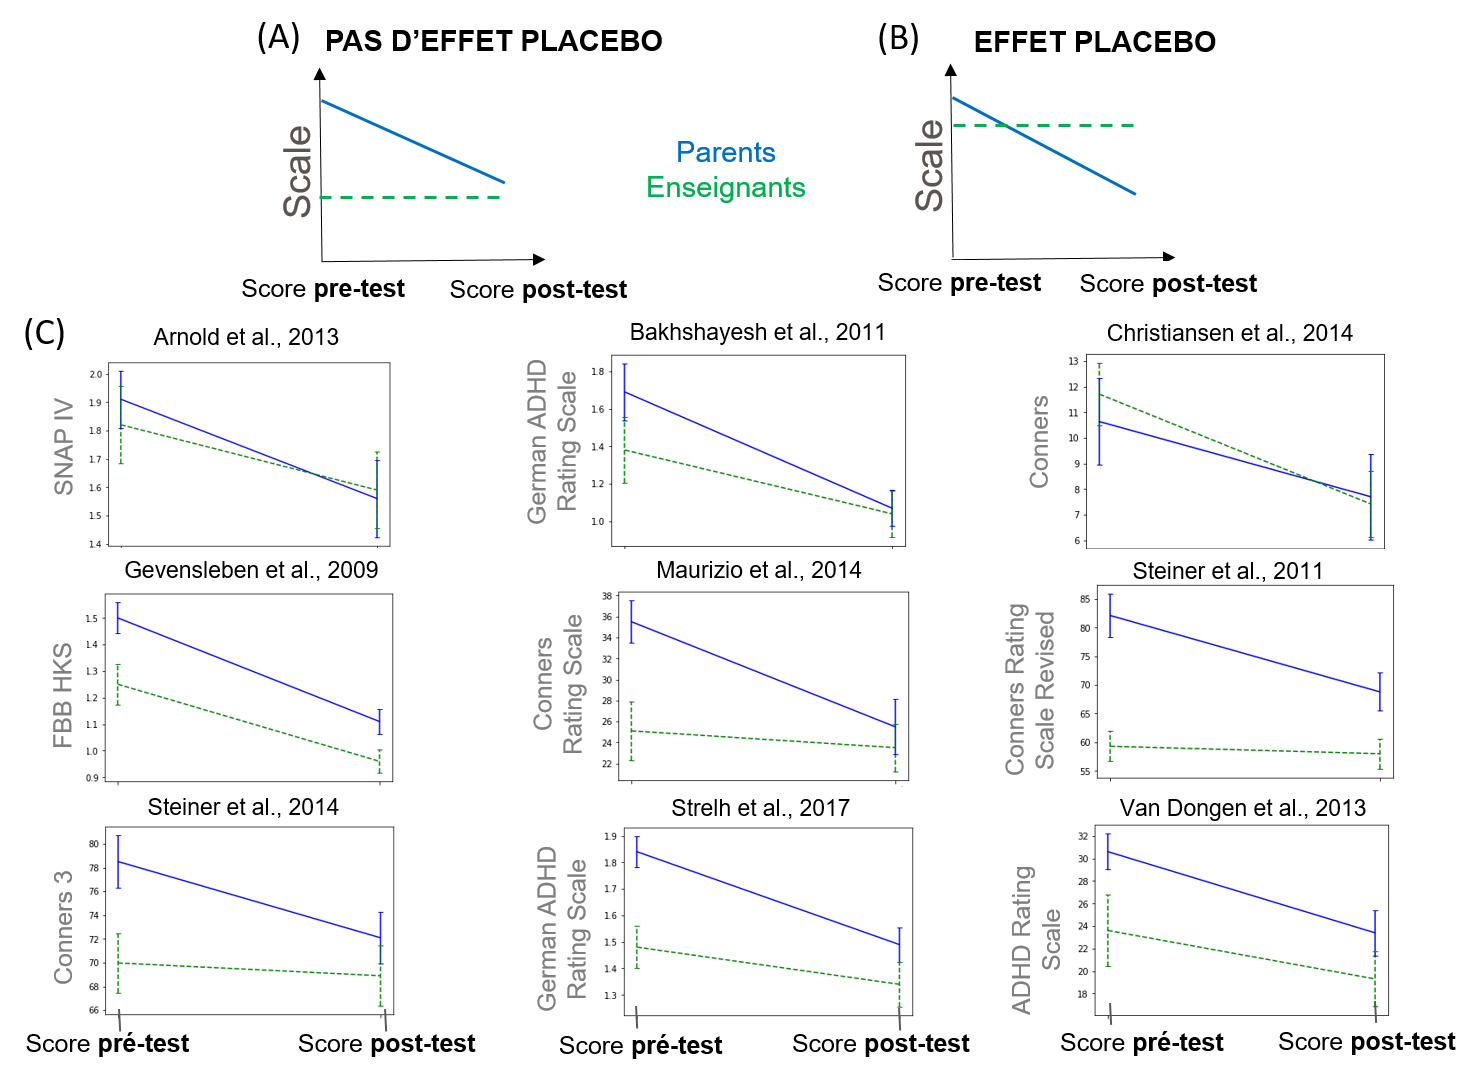
\includegraphics[width=1\linewidth]{figures/chapter-3/factors-pblind-discussion} 
  \caption[Comparaison des scores cliniques attribués aux enfants par les parents et les enseignants à pré et post-test.]{Scores à pré-test et post-test ($\pm$ erreur type) donnés par les parents (\gls{mprox}) en bleu et les enseignants (\gls{pblind}) en pointillés verts. 
	Deux hypothèses sur des données hypothétiques : en \textbf{A} pas d'effet placebo, les enseignants notent moins de symptômes du \gls{tdah} donc la difference entre pré et post-test est faible
	et en \textbf{B} effet placebo, les enseignants observent autant de symptômes à pré-test que les parents mais pas autant d'amélioration. En \textbf{C} résultats sur des données réelles : 
	évolution des scores attribués par les parents et enseignants entre pré- et post-test dans les études qui satisfont le critère d'inclusion de \citeauthor{Cortese2016} 
	et qui donnent les scores sur les mêmes échelles pour les deux types d'évaluateurs.}
  \label{Figure:factors_pblind_discussion}
\end{figure}

Ces différences d'évaluation entre parents et enseignants ont été étudiées à de multiples reprises \citep{Sollie2013, Narad2015, Minder2018}, montrant que 
ces derniers sont plus susceptibles de sous-estimer la sévérité des symptômes du \gls{tdah} chez l'enfant, surtout chez les plus jeunes. Par conséquent, les 
enseignants sont peut-être simplement moins capables d'observer un changement clinique durant la durée du traitement. Par ailleurs, les scores entre enseignants 
sont plus variables que ceux entre parents, ce qui peut en partie expliquer le faible \gls{es} (aussi bien intra que inter-groupes) calculé pour les évaluateurs
\gls{pblind}. Ainsi pour conclure, recourir aux évaluateurs \gls{pblind} pour estimer l'effet placebo n'apparait pas comme étant un choix approprié. 

Une autre façon de mettre en évidence un éventuel effet placebo est de se rapporter au \gls{dt} présenté à la Figure~\ref{Figure:factors_decision_tree}. Le 
\textit{root node} divise l'ensemble des données en deux parties : d'une part un sous arbre est créé avec 46 observations correspondant aux évaluateurs
\gls{mprox} et d'autre part, 21 observations correspondant aux évaluateurs \gls{pblind}. Si les différences observées entre ces deux types d'évaluateurs est due à l'effet
placebo, il serait attendu que le sous-arbre des observations \gls{mprox} comporte des facteurs liés à la perception de l'implication dans le traitement. En effet, dans cette
partie de l'arbre on trouve bien le facteur "durée du traitement", mais qui ne va pas dans la direction corroborant l'effet placebo : intuitivement, 
il est attendu que plus le traitement est long, plus l'effet placebo est important et plus l'\gls{es}-intra-groupe est élevé, or ici l'inverse est observé ce qui
contredit l'hypothèse. 

Ainsi, ces résultats suggèrent que les évaluateurs \gls{pblind} peuvent difficilement être utilisés pour quantifier l'effet placebo étant donné qu'ils paraissent
plus aveugles aux symptômes qu'au traitement. Etant donné que la mise en place de protocoles de \textit{sham}-\gls{nfb} éthiquement \citep{Holtmann2014} et techniquement 
\citep{Birbaumer1991} faisables est très difficile, il est nécessaire d'avoir recours à une méthode alternative et objective acceptable pour juger de l'efficacité du traitement 
\citep{World-Medical-Association2000}. Une analyse robuste envisageable serait d'étudier les neuromarqueurs collectés durant le traitement par \gls{nfb} pour démontrer que les 
patients contrôlent effectivement le neuromarqueur, qu'ils apprennent (c'est à dire que le contrôle du neuromarqueur s'intensifie avec le temps), et que cet apprentissage conduit 
à une réorgarnisation cérébrale durable. Ce genre d'analyse a été menée pour certaines études et conduit à des résultats favorables mais n'est pas 
systématique \citep{Arns2014}. Si aucune évolution du neuromarqueur n'est observée au cours du traitement alors que les évaluateurs \gls{mprox} notent une amélioration clinique 
des symptômes, on pourrait conclure que l'effet placebo joue un rôle dans ces résultats.

\subsection{Comparaison avec les résultats de Bussalb et al., 2019b}

L'analyse présentée dans ce chapitre est la mise à jour des résultats de \citet{Bussalb2019clinical}. Etant donné qu'un nombre encore limité d'études
d'efficacité est disponible sur le \gls{nfb} appliqué aux enfants \gls{tdah}, les analyses telles que les méta-analyses et la \gls{saob} doivent être régulièrement mises
à jour afin d'obtenir des résultats stables comme discuté en \ref{meta_analysis_update}.

\subsubsection{Différences avec les résultats de Bussalb et al., 2019b}
\citet{Bussalb2019clinical} présente des résultats obtenus sur des études publiées avant le 12 février 2018, ce qui correspond à 33 études (67 observations). La mise 
à jour décrite dans ce chapitre porte ce nombre à 41, augmentant ainsi la robustesse des
résultats. Malheureusement, tous les facteurs exclus dans l'analyse antérieure le sont également avec cette mise à jour et la validation par
un \gls{irb} est en plus rejetée.

Les différences entre \citet{Bussalb2019clinical} et sa mise à jour présentée dans ce chapitre sont mises en évidence à la 
Table~\ref{Table:table_factors_analysis_results_summary_update}.

\begin{table}[h!]
  \centering
  \caption[Comparaison entre les résultats de la \gls{saob} de \citet{Bussalb2019clinical} et de sa mise à jour.]{Resultats des mises à jour de la régression linéaire pondérée (\gls{wls}), de la régression linéaire régularisée (\gls{lasso}) et de l'arbre de décision (\gls{dt})
	comparés à ceux de \citet{Bussalb2019clinical}. Pour la \gls{wls}, une $p$-value $<$ 0.05 
	(en gras) signifie que le coefficient du facteur correspondant est significativement différent de 0. Pour le \gls{lasso}, les facteurs dont les coefficients sont non mis à 0 (en gras) sont 
	sélectionnés. Pour l'arbre de décision, la place du facteur dans l'arbre est indiquée. Pour les deux premières colonnes, quand la valeur du coefficient est négative le facteur 
	correspondant pourrait mener à de meilleurs résultats du \gls{nfb}. Les valeurs en vert correspondent aux valeurs devenues significatives après la mise à jour de \citet{Bussalb2019clinical}; les valeurs
	en rouges correspondent aux valeurs ayant perdu la significativité après la mise à jour.}
  \begin{center}
\small 
\begin{tabular}{ p{3cm} p{3cm} p{3cm} p{2cm} p{2cm} p{2cm}}
\toprule
\multicolumn{2}{c}{ \shortstack{Variables \\ indépendantes (facteurs)} } & \shortstack{ Coefficients \\ trouvés par \gls{wls} \\ ($p$-value) } & \shortstack{ Coefficients \\ trouvés par \\ \gls{lasso} } & \shortstack{Place \\ sur le \\ \gls{dt}} \\
\midrule
\multirow{ 3}{*}{ \textit{Méthodologiques} } & \gls{pblind} & \hskip 0.12in\textbf{0.15 (0.015)} & \hskip 0.12in\textbf{0.086} & \textbf{\textit{root node}} \\ 
& randomisation & \hskip 0.12in0.013 (0.840) & \hskip 0.12in\textcolor{red}{0.00} & / \\   
\midrule
\multirow{ 3}{*}{ \textit{Population} } & age max & \hskip 0.08in-0.10 (0.106) & \hskip 0.12in0.00 & / \\
& age min & \hskip 0.12in0.056 (0.43) & \hskip 0.12in0.00 & / \\
& prise de médicaments & \hskip 0.08in-0.026 (0.72) & \hskip 0.12in0.00 & / \\
\midrule
\multirow{ 9}{*}{ \textit{ \shortstack{Implementation \\ du \gls{nfb}} } } & nombre de sessions & \hskip 0.08in\textbf{-0.19 (0.025)} & \hskip 0.12in0.00 & \textcolor{red}{/} \\
& durée de la session & \hskip 0.08in\textcolor{red}{-0.13 (0.16)} & \hskip 0.12in0.00 & \textcolor{green}{\textbf{2$^{eme}$ noeud}} \\
& durée du traitement & \hskip 0.12in\textbf{0.39 (0.00)} & \hskip 0.12in\textbf{0.098} & \textbf{2$^{eme}$ et 3$^{eme}$ noeuds} \\
& fréquence des sessions & \hskip 0.12in0.027 (0.690) & \hskip 0.08in\textbf{-0.055} & \textbf{2$^{eme}$ noeud} \\ 
& \gls{smr} & \hskip 0.12in0.12 (0.067) & \hskip 0.12in0.00 & / \\
& augmentation de beta en central & \hskip 0.12in0.087 (0.32) & \hskip 0.12in\textcolor{green}{\textbf{0.026}} & / \\  
& diminution de theta & \hskip 0.08in-0.095 (0.39) & \hskip 0.12in0.00 & / \\
& \gls{scp} & \hskip 0.08in-0.14 (0.30) & \hskip 0.12in0.00 & / \\ 
& phase de transfert & \hskip 0.12in\textbf{0.33 (0.001)} & \hskip 0.12in\textcolor{green}{\textbf{0.079}} & \textcolor{green}{\textbf{1$^{er}$ noeud}} \\
\midrule
\multirow{ 2}{*}{ \textit{ \shortstack{Qualité de \\ l'acquisition} } } & plus d'une électrode d'enregistrement & \hskip 0.08in\textcolor{red}{-0.083 (0.20)} & \hskip 0.08in\textbf{-0.030} & / \\ 
& \gls{eeg} qualité 2 & \hskip 0.08in\textbf{-0.28 (0.00)} & \hskip 0.08in\textbf{-0.037} & \textcolor{red}{/} \\ 
\midrule
\multirow{ 2}{*}{ \textit{Qualité du signal} } & \gls{eog} rejet ou correction & \hskip 0.08in\textcolor{red}{-0.10 (0.164)} & \hskip 0.08in\textcolor{green}{\textbf{-0.0046}} & \textcolor{green}{\textbf{1$^{er}$ noeud}} \\ 
& Rejet des artefacts basé sur l'amplitude & \hskip 0.12in0.14 (0.058) & \hskip 0.12in0.00 & / \\   
\bottomrule
\end{tabular}
\end{center}
  \label{Table:table_factors_analysis_results_summary_update}
\end{table}

Les résultats obtenus sont globalement cohérents avec ceux présentés dans \citet{Bussalb2019clinical}. Les caractéristiques de la population n'ont toujours pas d'influence, ni
le type de protocole utilisé. Il en va de même pour l'influence positive de l'intensité du traitement et les moins bons résultats obtenus avec les évaluateurs \gls{pblind} qui sont
retrouvés par le même nombre de méthodes. 

Les différences notables concernent la qualité de l'\gls{eeg} égale à deux et la présence d'une phase de transfert. En effet, suite à la mise à jour de \citet{Bussalb2019clinical}, 
la qualité de l'\gls{eeg} égale à deux 
n'est plus identifiée par le \gls{dt}, diminuant ainsi la confiance quant à son impact sur l'efficacité du \gls{nfb}. Par ailleurs, bien que ce facteur soit intéressant, sa définition, 
donnée en \ref{choix_des_facteurs}, manque de précision 
du fait du peu d'informations disponibles sur le matériel utilisé par les études. Ainsi, afin d'évaluer au mieux son influence, les études devraient fournir 
davantage d'informations.

A l'inverse la présence d'une phase de transfert est désormais sélectionnée par les trois méthodes.

\subsubsection{Etude de l'évolution du nombre de méthodes sélectionnant un facteur entre les résultats de \citet{Bussalb2019clinical} et ceux de sa mise à jour} \label{evolution_methods}
Afin de mettre évidence la fluctuation des résultats, la même approche que celle décrite en \ref{meta_analysis_update} est suivie ici : l'évolution du nombre de méthodes de régression pour 
lesquelles un facteur est sélectionnné au fur et à mesure de l'ajout,
selon leur année de publication, des nouvelles études mettant à jour \citet{Bussalb2019clinical} est étudiée. 

Il a été decidé de s'intéresser à l'évolution des résultats en prenant comme origine ceux présentés dans \citet{Bussalb2019clinical} car le nombre d'observations y est déjà faible (67) compte tenu du nombre 
de variables indépendantes (19) : effectuer la \gls{saob} sur moins d'observations conduirait à des résultats peu fiables. 

Les facteurs dont l'évolution est illustrée en 
Figure~\ref{Figure:factors_evolution_with_update} ont été choisis d'une part, car chacun a été sélectionné par un nombre de méthodes différent suite à l'analyse décrite en \ref{saob_results}
et dont les résultats sont résumés à la Table~\ref{Table:table_factors_analysis_results_summary_number_of_factors} et, d'autre part, pour les raisons suivantes :
\begin{itemize}
\item \textsl{la durée du traitement :} sélectionné par trois méthodes dans \citet{Bussalb2019clinical}, ce facteur l'est également suite à la mise à jour présentée en \ref{saob_results},
il est donc intéressant de savoir si le nombre de méthodes a changé au cours de l'ajout des nouvelles études,
\item \textsl{la qualié de l'\gls{eeg} égale à 2 :} sélectionné par trois méthodes dans \citet{Bussalb2019clinical}, seules deux méthodes l'identifient suite à la mise à jour.
L'analyse de son évolution au cours du temps permettra de déterminer si elle se stabilise ou non,
\item \textsl{le nombre de sessions :} ce paramètre a été identifié par deux méthodes dans \citet{Bussalb2019clinical}, mais ce nombre est de un suite à la mise à jour des résultats.
Etant donné que la valeur de ce facteur est très discutée dans la littérature comme rappelé en \ref{discussion_factors}, il semble judicieux d'étudier ce facteur plus précisément,
\item \textsl{le protocole \gls{smr} :} ce facteur n'est sélectionné par aucune méthode, aussi bien dans \citet{Bussalb2019clinical} que dans sa mise à jour. Il a été choisi arbitrairement
parmi les protocoles d'entrainenemt retourné par aucune méthode pour mettre en évidence une éventuelle fluctuation au cours du temps de ce type de facteur qui parait intuivement central comme
discuté en \ref{discussion_factors}.
\end{itemize}

Afin de mettre en évidence le nombre croissant d'observations avec l'ajout de nouvelles études dans la \gls{saob}, le nombre d'observations 
incluses dans chaque nouvelle étude ajoutée (NO) ainsi que le nombre cumulatif d'observations (NOC) sont donnés sur les axes des abscisses supérieurs.
Ils sont obtenus de la façon suivante : $\text{NOC}(k) = \text{NOC}(k - 1) + \text{NO}(k)$, avec $k$ l'indice de l'étude incluse
allant de $1$ à $K$, avec $K$ le nombre total d'études incluses.

\begin{figure}[h!]
  \centering
	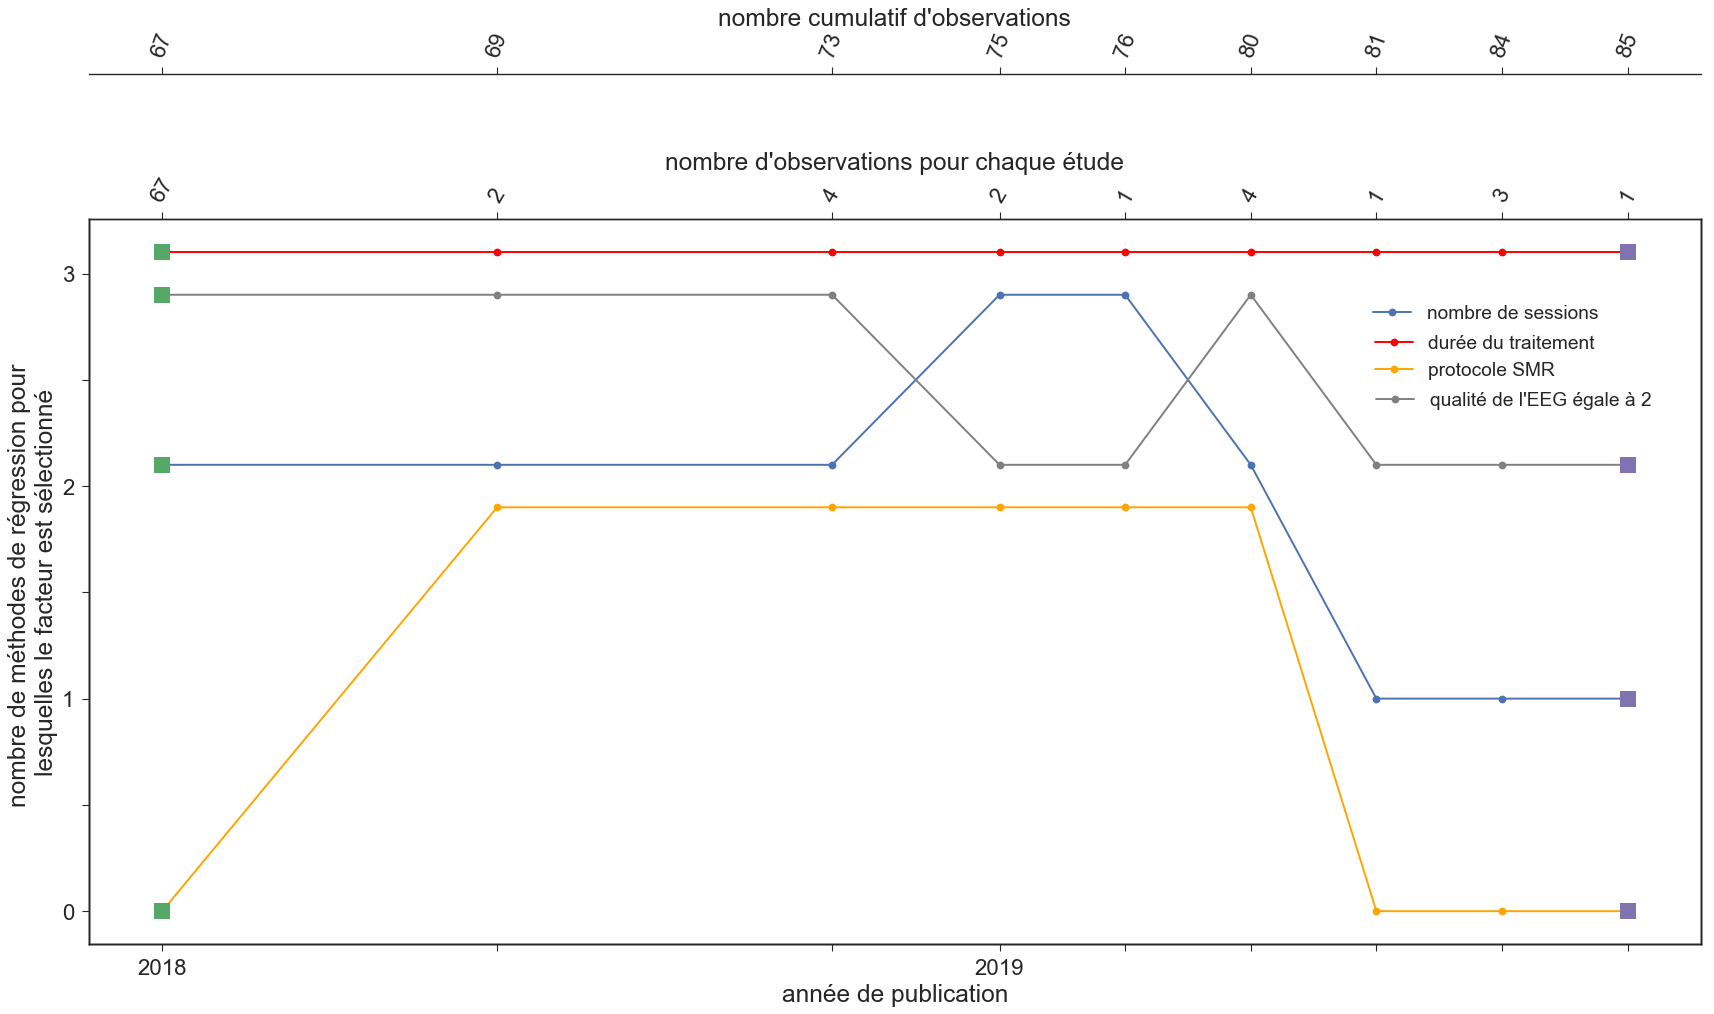
\includegraphics[width=1\linewidth]{figures/chapter-3/factors-evolution-with-update} 
  \caption[Evolution du nombre de méthodes de régression pour lesquelles les facteurs sont sélectionnés au fur et à mesure de l'ajout de nouvelles études.]{Evolution du nombre de méthodes de régression pour lesquelles les facteurs sont sélectionnés au fur et à mesure de l'ajout des études mettant à jour \citet{Bussalb2019clinical}.
	La courbe rouge correspond au facteur "durée du traitement", la grise à "la qualité de \gls{eeg} égale à 2", la bleue au "nombre de sessions", la orange au "protocole \gls{smr}". 
	Les carrés verts représentent les résultats de \citet{Bussalb2019clinical} et les violets ceux de la mise à jour de cet article présentée en \ref{saob_results}.
	Le nombre d'observations incluses dans chaque nouvelle étude ajoutée ainsi que le nombre cumulatif d'observations sont donnés sur les axes des abscisses supérieurs.
	La façon dont est calculé le nombre cumulatif d'observations incluses est décrite en \ref{evolution_methods}.}
  \label{Figure:factors_evolution_with_update}
\end{figure}

Au cours de l'ajout des huit études représenté en Figure~\ref{Figure:factors_evolution_with_update}, aucune variation du nombre de méthodes sélectionnant la durée du traitement (en rouge) 
n'est à noter :
ce résultat semble s'être stabilisé. Par contre, le nombre de méthodes identifiant le nombre de sessions (en bleu) et la qualité de l'\gls{eeg} égale à 2 (en gris) oscille, rendant plus 
compliqué de conclure quant à l'influence de ces facteurs sur l'efficacité du \gls{nfb} appliqué aux enfants \gls{tdah}. Les résultats concernant le protocole \gls{smr} varient
également et de manière plus importante, en passant d'aucune méthode à deux méthodes puis en retombant à zéro méthode.

Ces courbes montrent donc que certains résultats ne sont pas figés : ils vont fluctuer jusqu'à se stabiliser quand un grand nombre d'observations sera disponible. 

Ainsi, pour que la \gls{saob} puisse apporter des indications fiables quant au design d'une étude évaluant l'efficacité du \gls{nfb} appliqué aux enfants \gls{tdah}, elle doit être 
régulièrement mise à jour. 

\section{Conclusion} \label{conclusion_saob}

La \gls{saob} a permis de mettre en évidence que l'intensité du traitement contribue à l'efficacité du \gls{nfb}, ce qui va dans le sens de ce qui est connu à propos de 
la théorie de l'apprentissage \citep{Mowrer1960} : un entrainement plus intense mène à une efficacité clinique augmentée. 

Dans une plus faible mesure, la \gls{saob} a permis d'identifier un facteur lié à la qualité du signal et un autre au matériel d'acquisition de l'\gls{eeg} comme ayant une influence positive 
sur l'efficacité du \gls{nfb}, ce qui indique fortement qu'elle est liée à un mécanisme d'action basé sur la modulation de l'\gls{eeg}. Toutefois, le paramètre lié à la qualité du signal 
souffre du peu d'informations fourni par les études à ce sujet, mais étant donné l'appel de
communauté du \gls{nfb} à être le plus transparent possible quant au matériel utilisé \citep{Ros2019}, il sera sans doute possible d'étudier plus précisément
son impact lors de futures analyses.

Alors que les trois facteurs précédents sont en faveur de l'efficacité du \gls{nfb}, l'influence négative de la présence d'une phase de transfert sur laquelle sont d'accord les trois méthodes, 
démontre plutôt un effet placebo. 

Bien que ces résultats contribuent certainement au débat, ce travail montre également que l'ultime démonstration de la preuve de l'efficacité du \gls{nfb}
appliqué aux enfants \gls{tdah} n'est pas encore atteinte, étant donné que les évaluations des enseignants ont été en partie invalidées comme indicatrices de 
l'effet placebo. Par conséquent, se référer aux résultats des évaluateurs \gls{pblind} pour mettre en évidence la spécificité de l'efficacité clinique n'est pas 
recommandé : il serait préférable d'avoir recours au \textit{sham}-\gls{nfb} et à l'analyse des changements de l'\gls{eeg} en fonction des neuromarqueurs entrainés.

Comme l'a montré la mise à jour des résultats de la \gls{saob}, les conclusions de cette analyse peuvent encore évoluer. Pour qu'elles se stabilisent, 
davantage d'observations sont nécessaires : une façon de résoudre ce problème serait d'inclure dans la \gls{saob} tous les articles sur l'efficacité du 
\gls{nfb} sans tenir compte de son application. Une telle \gls{saob} n'aurait pas pour but de déterminer les facteurs ayant une influence sur 
l'efficacité du \gls{nfb} sur les enfants \gls{tdah} comme c'est le cas dans ce chapitre, mais ceux ayant une influence en général sur 
l'efficacité du \gls{nfb}, quelle que soit son application. Toutefois, les résultats de l'analyse menée ici donne tout de même des pistes pour améliorer 
la performance du \gls{nfb} appliqué aux enfants \gls{tdah}. 

Au vu du nombre important d'études publiées sur le \gls{nfb} appliqué aux enfants \gls{tdah}, certains facteurs vont pouvoir finir par être inclus dans la \gls{saob}, comme par exemple 
l'individualisation du protocole de \gls{nfb} qui semble prometteuse. Le chapitre suivant va justement s'intéresser à la distribution d'un marqueur de l'attention, 
le \gls{tbr}, au sein d'une large population afin de déterminer si une personnalisation basée sur ce neuromarqueur est envisageable.




 